%!TEX root = ../thesis.tex
%*******************************************************************************
%****************************** Introduction *********************************
%*******************************************************************************

\chapter{Introduction}

Over the past decade, artificial intelligence (AI) has undergone a transformative evolution, driven by groundbreaking advancements in generative modeling and self-supervised learning (SSL). These two fields have redefined our ability to model complex data distributions and leverage vast amounts of unlabeled data, leading to significant breakthroughs in areas such as media synthesis \cite{karras2019style, ramesh2021zero, esser2021taming, kong2020diffwave}, multimodal learning \cite{radford2021learning, xu2021videoclip, wang2022image}, and scientific discovery \cite{jumper2021highly, stokes2020deep, rives2021biological, zhang2021unified}.

Generative modeling focuses on learning the underlying probability distributions of data to create realistic and diverse samples. Innovations such as Generative Adversarial Networks (GANs) \cite{goodfellow2014generative}, diffusion models \cite{ho2020denoising, song2021score}, and normalizing flows \cite{rezende2015variational, papamakarios2019normalizing} have set new benchmarks in quality and applicability, enabling realistic image generation \cite{karras2019style}, lifelike video creation \cite{esser2021taming}, natural-sounding audio synthesis \cite{kong2020diffwave}, and text-to-image generation \cite{ramesh2021zero}. Beyond creative media, these models play a critical role in scientific applications, such as protein structure prediction \cite{jumper2021highly, baek2021accurate}, AI-assisted drug discovery \cite{stokes2020deep, gentile2020deep}, and materials science \cite{butler2018machine}, where they accelerate research by generating novel molecules and exploring chemical spaces. Furthermore, they address challenges in inverse problems, including super-resolution \cite{saharia2022image, wang2024sinsr} and inpainting \cite{suvorov2022resolution, lugmayr2022repaint}.

Self-supervised learning, on the other hand, has emerged as a powerful approach to harness the vast reservoirs of unlabeled data by uncovering its inherent structure. SSL enables models to learn meaningful representations that are crucial for downstream tasks, often serving as the backbone of state-of-the-art systems across diverse domains. These representations can be extracted using generative methods, which model the data distribution, or discriminative methods, such as contrastive learning \cite{chen2020simple}, which focus on distinguishing between similar and dissimilar data samples.

Self-supervised learning has had a profound impact on foundational technologies. In natural language processing, it powers groundbreaking models like BERT \cite{devlin2018bert} and GPT \cite{brown2020language}, which underpin conversational AI and advanced language understanding systems. In computer vision, SSL reduces dependence on labeled data while delivering robust, scalable visual representations, driving improvements in tasks like object recognition and image segmentation. These advancements underscore SSL’s versatility and its pivotal role in advancing AI across domains and modalities. Additionally, SSL has been transformative in multimodal learning, enabling seamless alignment and integration across modalities such as text, images, and audio. This capability has unlocked advanced tasks like generating descriptive image captions \cite{hossain2019comprehensive}, synchronizing audio with video \cite{arandjelovic2017look}, retrieving relevant content across formats \cite{sun2019videobert}, and enhancing representation learning for multimodal datasets \cite{radford2021learning}.

In this thesis, we focus on the theoretical and computational aspects of generative modeling and generative self-supervised learning. To provide the necessary background, the remainder of this introduction is divided into two sections: an overview of generative modeling (\ref{intro:generative_modeling}) and an overview of self-supervised learning (\ref{intro:ssl}).


\section{Generative Modeling}\label{intro:generative_modeling}
\subsection{The Problem of Generative Modeling}

Generative modeling sits at the forefront of machine learning, enabling us to capture the underlying structure of complex data and generate new, realistic samples. Whether it's creating lifelike images, composing music, or designing novel molecules, generative models aim to understand and replicate the distribution of data they're trained on.

Formally, let's consider a dataset \( \mathcal{D} = \{ \mathbf{x}_1, \mathbf{x}_2, \dots, \mathbf{x}_N \} \subset \mathbb{R}^d \), comprising \( N \) independent samples drawn from an unknown data-generating distribution \( P(X) \), which we refer to as the \textit{target distribution}. The central goal of generative modeling is to create a model that approximates \( P(X) \) as closely as possible based solely on these samples.

To learn the distribution \( P(X) \), we seek a computationally tractable approximation \( \hat{P}(X) \) based on the dataset \( \mathcal{D} \) and our assumptions about \( P(X) \). We measure how close \( \hat{P}(X) \) is to \( P(X) \) using a divergence \( D(\hat{P}(X), P(X)) \), such as the Kullback-Leibler divergence or the Wasserstein distance. Our goal is to minimize this divergence:

\[
P^{\ast}(X) = \arg \min_{\hat{P}(X)} D(\hat{P}(X), P(X)).
\]

Typically, we parameterize \( \hat{P}(X) \) with a finite-dimensional vector \( \theta \in \mathbb{R}^p \) for some $p>0$, forming a family of models \( P_{\theta}(X) \) and transforming the problem into optimizing over parameters:

\[
\theta^* = \arg \min_\theta D(P_{\theta}(X), P(X)).
\]

For practicality, \( P_{\theta}(X) \) must be computationally tractable; we should be able to efficiently sample from it or evaluate its probability density function. Different generative modeling approaches balance tractability and fidelity to \( P(X) \), leading to various methods suitable for different applications.

By tackling this problem, we aim not only to reproduce the data we observe but also to uncover the underlying mechanisms that generate it. This deep understanding empowers us to create models that can generate new, unseen data that is indistinguishable from real-world samples, thereby expanding the horizons of what machines can learn and create.

\subsection{Why Deep Learning for Generative Modeling?}

Non-parametric methods such as Kernel Density Estimation (KDE) have been widely used for modeling probability distributions in low-dimensional settings due to their flexibility in estimating the underlying density without assuming a specific parametric form \cite{silverman1986density}. However, scaling KDE to high-dimensional data is problematic. The sample complexity of KDE scales exponentially with the number of feature dimensions \( d \), making it impractical for high-dimensional tasks \cite{wasserman2006all}. Specifically, as per \cite{scott2015multivariate}, the number of samples \( n \) required to achieve a target estimation error \( \varepsilon \) must satisfy the following condition:

\[
n \geq \mathcal{O}\left(\varepsilon^{-\frac{4 + d}{4}}\right).
\]

\noindent This exponential dependence on \( d \) implies that even for moderate dimensions, the required sample size becomes infeasibly large, rendering KDE and similar methods ineffective for generative modeling in high dimensions.

In many real-world applications, however, data does not uniformly occupy the high-dimensional ambient space but is concentrated near a lower-dimensional manifold—a concept known as the \emph{manifold hypothesis} \cite{fefferman2016testing}. For example, natural images, although high-dimensional when represented by pixel values, often lie on manifolds of much lower intrinsic dimensionality due to dependencies and correlations among pixels \cite{roweis2000nonlinear}. This implies that the effective complexity of the data is determined by the manifold's dimension \( k \), where \( k \ll d \).

While the manifold hypothesis suggests a reduction in effective dimensionality, leveraging this property requires models that can explicitly capture the underlying manifold structure. Non-parametric methods like KDE do not inherently account for the manifold and treat each dimension independently, failing to exploit the dependencies among features \cite{tenenbaum2000global}. As a result, they still suffer from high sample complexity despite the data's lower intrinsic dimensionality.

Parametric models with appropriate inductive biases can overcome this limitation by incorporating assumptions about the data's structure into the learning process. Deep learning architectures are particularly well-suited for this task due to their ability to integrate domain-specific inductive biases through their design \cite{lecun2015deep}. For instance, Convolutional Neural Networks (CNNs) employ local connectivity and weight sharing to capture spatial hierarchies and local patterns in image data \cite{lecun1998gradient}. Similarly, Recurrent Neural Networks (RNNs) are designed to model temporal dependencies in sequential data \cite{hochreiter1997long}.

By aligning model architecture with the intrinsic properties of the data manifold, deep learning models effectively reduce the hypothesis space to functions consistent with the data's structure, enhancing learning efficiency and reducing the required number of samples \cite{poggio2017theory}. This structural approach explains why deep learning–based methods have become indispensable for generative modeling in high dimensions \cite{goodfellow2016deep,kingma2013auto}.

In the past decade, deep learning has introduced flexible architectures that can effectively learn complex data distributions. This chapter reviews six main types of generative models: Generative Adversarial Networks (GANs), Variational Auto-encoders (VAEs), Normalizing Flows, Auto-Regressive Models, Energy-Based Models, and Diffusion Models, each with unique strengths and limitations.

\subsection{Generative Adversarial Networks (GANs)}\label{sec:gans}

Introduced by Goodfellow et al. \cite{goodfellow2014generative}, Generative Adversarial Networks (GANs) consist of two neural networks: a \textit{generator} \( G \) and a \textit{discriminator} \( D \), trained simultaneously in a minimax game. The generator maps samples \( \mathbf{z} \) from a simple prior distribution \( P(Z) \) (e.g., a standard normal distribution) to the data space \( \mathbb{R}^d \), producing synthetic data \( G(\mathbf{z}) \). The discriminator outputs a probability \( D(X) \in [0,1] \) indicating whether a sample \( X \) is real (from the training data) or generated (from \( G \)).

\textsc{Training Objective.} The training objective is formulated as a two-player minimax game with the value function \( V(D, G) \):
\[
\min_{G} \max_{D} V(D, G) = \mathbb{E}_{X \sim P(X)} [\log D(X)] + \mathbb{E}_{Z \sim P(Z)} [\log (1 - D(G(Z)))]
\]
where \( P(X) \) is the target distribution represented by the training set \( \mathcal{D} \).


GANs are trained through an adversarial process where the generator and discriminator are updated iteratively to improve against each other. The discriminator \( D \) learns to better distinguish real data from generated data, while the generator \( G \) aims to produce data that can fool \( D \). This training continues until the generator produces samples indistinguishable from real data (\( P_G(X) = P(X) \)).

There are various formulations of the value function designed to enhance training stability and performance. For instance, the Wasserstein GAN (WGAN) \cite{arjovsky2017wasserstein} modifies the original objective using the Earth Mover's distance to address issues like mode collapse and improve convergence.

\textsc{Strengths.} GANs have several notable strengths. One of their primary advantages is their ability to produce \textbf{high-quality samples} that are visually realistic and sharp, especially in image generation tasks (see Figure~\ref{fig:stylegan_samples}). Additionally, GANs offer \textbf{efficient sampling}; once the generator is trained, it can rapidly produce new samples through a single forward pass, without the need for iterative sampling procedures common in other generative models.

\begin{figure}[ht]
    \centering
    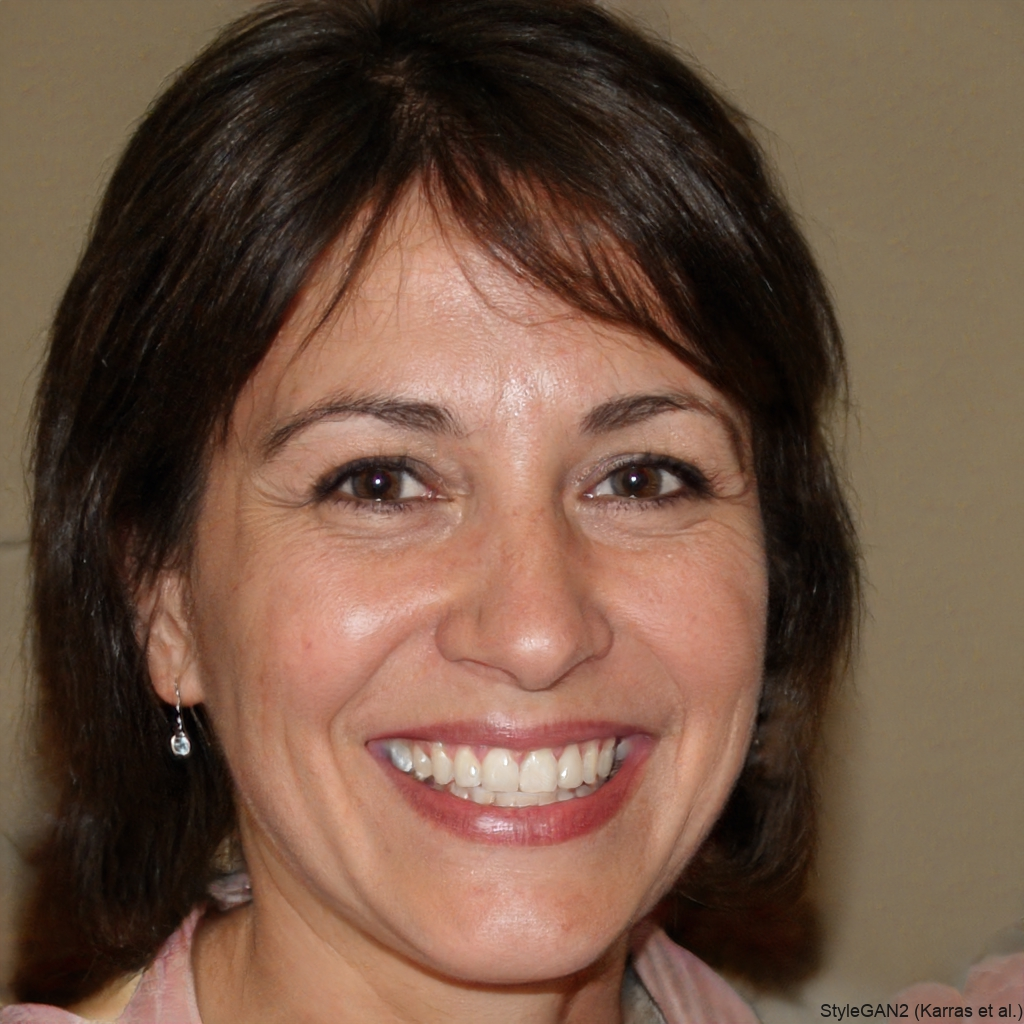
\includegraphics[width=0.32\textwidth]{introduction/figures/stylegan_example_1.jpeg}
    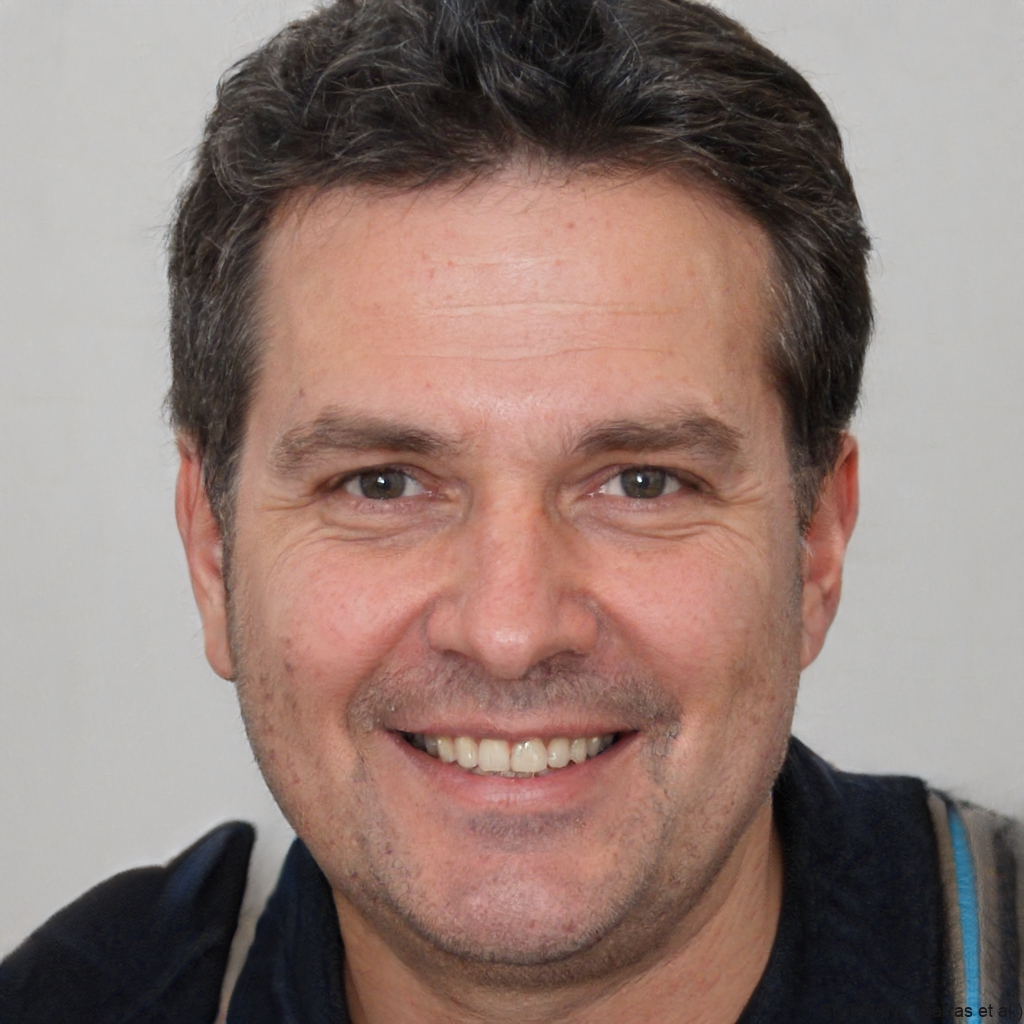
\includegraphics[width=0.32\textwidth]{introduction/figures/stylegan_example_2.jpeg}
    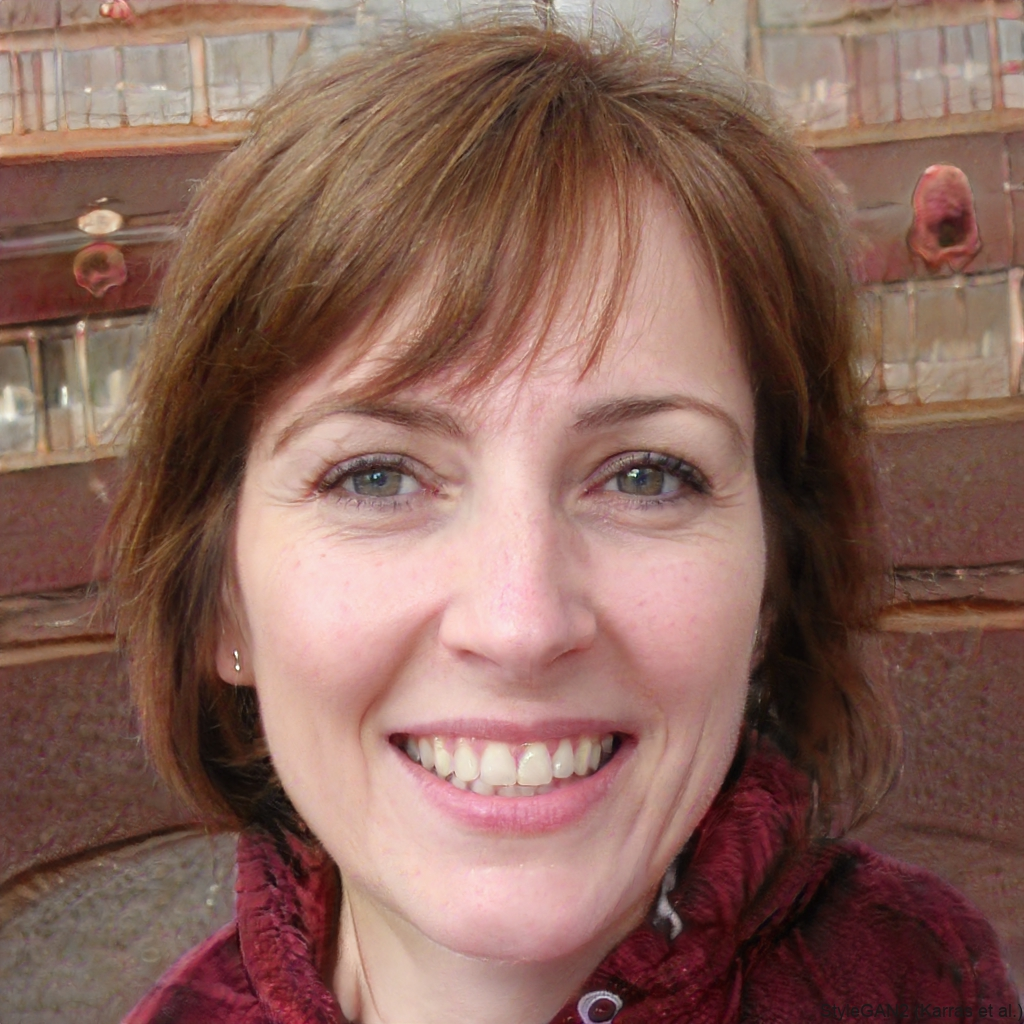
\includegraphics[width=0.32\textwidth]{introduction/figures/stylegan_example_3.jpeg}
    \caption{Samples generated by the StyleGAN model \cite{karras2019stylegan}. These high-resolution, realistic images demonstrate the capability of GANs to produce lifelike outputs.}
    \label{fig:stylegan_samples}
\end{figure}


\textsc{Weaknesses.} Despite their impressive capabilities, GANs come with a set of significant limitations that hinder their broader applicability. One of the most pressing challenges is their \textbf{training instability}, which stems from the adversarial nature of their setup. This instability often manifests in issues such as \textbf{mode collapse} \citep{arjovsky2017wasserstein}, where the generator fails to capture the diversity of the data distribution and instead produces limited varieties of samples—sometimes focusing on a single mode (see Figure~\ref{fig:mode_collapse}). This issue significantly impacts the utility of GANs, particularly in applications where diversity of the generated data is critical.

Another prominent challenge is the problem of \textbf{vanishing gradients} \citep{arjovsky2017wasserstein}. This occurs when the discriminator becomes too strong relative to the generator, leading to minimal gradient updates for the generator and stagnating its progress. Additionally, GANs are prone to \textbf{oscillatory behavior} during training, where the generator and discriminator fail to reach equilibrium, resulting in unstable or suboptimal convergence \citep{mescheder2018which}.

Moreover, GANs suffer from a fundamental limitation: they \textbf{do not provide an explicit density function} or a likelihood estimate for the generated data. This restricts their use in tasks requiring probabilistic interpretations, such as uncertainty quantification or anomaly detection, where an understanding of sample likelihoods is essential.

These challenges highlight the need for alternative or complementary generative modeling approaches, such as normalizing flows \citep{papamakarios2019normalizing} or diffusion models \citep{ho2020denoising}, which offer more stable training and explicit density estimation, enabling broader applicability and robustness across diverse tasks. However, GANs remain a valuable tool in scenarios where visual fidelity and sample quality are the primary objectives.

\begin{figure}[h!]
    \centering
    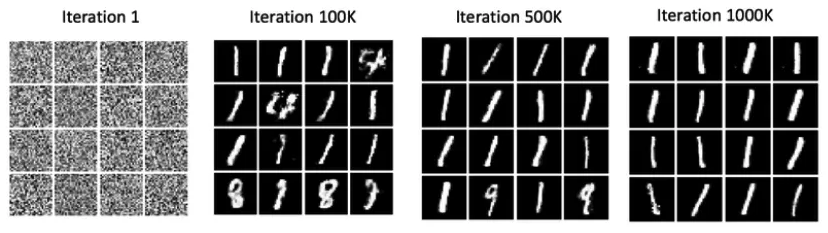
\includegraphics[width=0.8\textwidth]{introduction/figures/mode_collapse.png}
    \caption{Demonstration of mode collapse in GANs: A vanilla GAN trained on the MNIST dataset is expected to generate samples from all modes of the data distribution (i.e., all digits). However, as training progresses, the generator increasingly focuses on producing convincing samples of a single mode (i.e., the digit 1), illustrating the issue of mode collapse. This highlights the tendency of GANs to fail in capturing the diversity of the data distribution.}
    \label{fig:mode_collapse}
\end{figure}



\subsection{Variational Autoencoders (VAEs)}\label{sec:vae}

Variational Autoencoders (VAEs), introduced by \citet{kingma2013auto} and \citet{rezende2014stochastic}, are a powerful class of latent variable models. They aim to simultaneously learn a compact, low-dimensional latent representation of data and a generative process capable of synthesizing new samples. This combination makes VAEs a cornerstone of representation learning and probabilistic generative modeling.

VAEs rely on the assumption that observed data \(X \in \mathcal{X}\) is generated from unobserved latent variables \(Z \in \mathcal{Z}\) through a probabilistic generative process. This process is characterized by two key components. The latent variable \(Z\) is assumed to follow a simple prior distribution, typically a standard normal distribution:
\[
p_{Z}(\mathbf{z}) = \mathcal{N}(\mathbf{z}; \mathbf{0}, \mathbf{I}),
\]
which encourages compact and smooth representations in the latent space. The observed variable \(X\), conditioned on a latent sample \(\mathbf{z}\), follows a parameterized conditional density:
\begin{equation}
p_{X \mid Z, \theta}(\mathbf{x} \mid \mathbf{z}) = \mathcal{N}(\mathbf{x}; \mu_\theta(\mathbf{z}), \sigma_\theta^2(\mathbf{z}) \mathbf{I}),
\end{equation}\label{intro:eq:gaussian_reconstruction}

where the mean \(\mu_\theta(\mathbf{z}) \in \mathbb{R}^d\) and variance \(\sigma_\theta^2(\mathbf{z}) \in \mathbb{R}\) are outputs of a neural network (decoder) with parameters \(\theta\). These assumptions define the generative model: latent variables are sampled from the prior, and data is generated conditionally through the decoder network.

\textit{The Challenge of Marginal Likelihood Optimization.}  
The marginal log-likelihood of a data point \(\mathbf{x}\) under the stated model assumptions is given by:
\[
\log p_{X, \theta}(\mathbf{x}) = \log \int p_{X, Z, \theta}(\mathbf{x}, \mathbf{z}) \, d\mathbf{z} = \log \int p_{X \mid Z, \theta}(\mathbf{x} \mid \mathbf{z}) \, p_{Z}(\mathbf{z}) \, d\mathbf{z}.
\]

This integral is intractable because, for a given data point \(\mathbf{x}\), only a small region in the latent space \(\mathcal{Z}\) significantly contributes to the likelihood. This critical region corresponds to values of \(\mathbf{z}\) where the conditional likelihood \(p_{X \mid Z, \theta}(\mathbf{x} \mid \mathbf{z})\) is high, concentrating most of the reconstruction probability mass. Intuitively, this reflects the fact that each data point is typically explained by a specific combination of underlying generative factors, such as shape, texture, or orientation, which correspond to a small subset of the latent space. When attempting to estimate the integral using Monte Carlo sampling from the prior \(p_Z(\mathbf{z})\), the vast majority of samples fall outside this region and contribute negligibly to the likelihood. This leads to highly inefficient sampling and high-variance estimates, as reliable integration would require an impractically large number of samples.

If we could sample directly from the true posterior \(p_{Z \mid X, \theta}(\mathbf{z} \mid \mathbf{x})\), which focuses on this important region of the latent space, we could obtain reliable Monte Carlo estimates of the likelihood. However, the true posterior itself depends on the intractable marginal likelihood \(p_{X, \theta}(\mathbf{x})\), making direct computation impractical. This is where the variational approximation of the posterior comes into play.

\textit{Variational Approximation of the True Posterior.} To address this intractability, VAEs introduce a variational approximation \(q_{Z \mid X, \phi}(\mathbf{z} \mid \mathbf{x})\), modeled by a neural network (the encoder), to approximate the true posterior \(p_{Z \mid X, \theta}(\mathbf{z} \mid \mathbf{x})\). The variational distribution \(q_{Z \mid X, \phi}(\mathbf{z} \mid \mathbf{x})\) is parameterized as a Gaussian:
\[
q_{Z \mid X, \phi}(\mathbf{z} \mid \mathbf{x}) = \mathcal{N}(\mathbf{z}; \mu_\phi(\mathbf{x}), \mathrm{diag}(\sigma_\phi^2(\mathbf{x}))),
\]
where \(\mu_\phi(\mathbf{x}) \in \mathbb{R}^k\) and \(\sigma_\phi(\mathbf{x}) \in \mathbb{R}^k\) are outputs of the encoder network with parameters \(\phi\) and $k$ denotes the dimension of the latent space.

The encoder is trained to match the true posterior as closely as possible, ensuring that the critical region of the latent space is sampled effectively. This enables low-variance Monte Carlo estimates of the marginal likelihood via importance sampling. The variational approximation thus transforms an otherwise intractable optimization problem into a practical one, paving the way for the derivation of the evidence lower bound (ELBO), a tractable objective that can be efficiently optimized to jointly train the encoder and decoder.

\textit{Derivation of the Evidence Lower Bound (ELBO).} To address the intractability of directly optimizing the marginal log-likelihood \(\log p_{X,\theta}(\mathbf{x})\), the variational approximation \(q_{Z\mid X,\phi}(\mathbf{z} \mid \mathbf{x})\) is utilized. This approximation allows efficient sampling from the critical region of the latent space that contributes most to the likelihood. Rewriting the marginal log-likelihood gives:
\[
\log p_{X,\theta}(\mathbf{x}) 
\,=\,
\log 
\int 
q_{Z \mid X,\phi}(\mathbf{z} \mid \mathbf{x}) 
\frac{p_{X,Z,\theta}(\mathbf{x}, \mathbf{z})}{q_{Z \mid X,\phi}(\mathbf{z} \mid \mathbf{x})}
\, d\mathbf{z}.
\]
The term inside the integral represents an importance-weighted likelihood, where the variational distribution \(q_{Z \mid X,\phi}(\mathbf{z} \mid \mathbf{x})\) serves as the proposal distribution for efficiently sampling from the posterior. 

Applying Jensen's inequality to the logarithm of the expectation yields:
\[
\log p_{X,\theta}(\mathbf{x}) 
\,\geq\,
\mathbb{E}_{q_{Z \mid X,\phi}(\mathbf{z} \mid \mathbf{x})} 
\left[
\log \frac{p_{X,Z,\theta}(\mathbf{x}, \mathbf{z})}{q_{Z \mid X,\phi}(\mathbf{z} \mid \mathbf{x})}
\right].
\]
The right-hand side is defined as the \emph{Evidence Lower Bound} (ELBO), denoted as \(\mathrm{ELBO}(\theta, \phi)\). By construction, the ELBO provides a tractable lower bound on the marginal log-likelihood and serves as the objective for training VAEs. Substituting the joint probability \(p_{X,Z,\theta}(\mathbf{x}, \mathbf{z}) = p_{X \mid Z,\theta}(\mathbf{x} \mid \mathbf{z}) \, p_Z(\mathbf{z})\), the ELBO can be expressed as:
\[
\mathrm{ELBO}(\theta, \phi) 
\,=\,
\mathbb{E}_{q_{Z \mid X,\phi}(\mathbf{z} \mid \mathbf{x})}
\big[
\log p_{X \mid Z,\theta}(\mathbf{x} \mid \mathbf{z})
\big]
\;-\;
D_{\mathrm{KL}}
\big(q_{Z \mid X,\phi}(\mathbf{z} \mid \mathbf{x}) \,\|\, p_Z(\mathbf{z})\big).
\]

\noindent The ELBO consists of two terms:
\begin{enumerate}
    \item \textbf{Reconstruction Term:}  
    \[
    \mathbb{E}_{q_{Z \mid X,\phi}(\mathbf{z} \mid \mathbf{x})} 
    \big[\log p_{X \mid Z,\theta}(\mathbf{x} \mid \mathbf{z})\big],
    \]
    which encourages the generative model \(p_{X \mid Z,\theta}\) (decoder) to reconstruct the observed data \(\mathbf{x}\) accurately from the latent representation \(\mathbf{z}\).
    \item \textbf{KL Divergence Term:}  
    \[
    D_{\mathrm{KL}}(q_{Z \mid X,\phi}(\mathbf{z} \mid \mathbf{x}) \,\|\, p_Z(\mathbf{z})),
    \]
    which regularizes the approximate posterior \(q_{Z \mid X,\phi}\), ensuring that the learned latent representations are close to the prior \(p_Z\).
\end{enumerate}

Together, these terms balance accurate data reconstruction and latent space regularization. Maximizing the ELBO ensures the latent space encodes meaningful, generalizable representations while enabling robust reconstruction through the decoder.

\textit{Connection to the Marginal Log-Likelihood.} To further understand the role of the ELBO, the marginal log-likelihood can be decomposed as follows:
\[
\log p_{X,\theta}(\mathbf{x}) 
\,=\,
\mathrm{ELBO}(\theta, \phi)
\,+\,
D_{\mathrm{KL}}\big(q_{Z \mid X,\phi}(\mathbf{z} \mid \mathbf{x}) \,\|\, p_{Z \mid X,\theta}(\mathbf{z} \mid \mathbf{x})\big).
\]
The second term is the KL divergence between the approximate posterior \(q_{Z \mid X,\phi}\) and the true posterior \(p_{Z \mid X,\theta}\). This term is always non-negative, implying that \(\mathrm{ELBO}(\theta, \phi) \leq \log p_{X,\theta}(\mathbf{x})\). From this decomposition, it additionally becomes clear that maximizing the ELBO serves a dual purpose:
\begin{enumerate}
    \item It increases the lower bound on the marginal log-likelihood, improving the model's ability to explain the data.
    \item It minimizes the mismatch between the approximate posterior \(q_{Z \mid X,\phi}\) and the true posterior \(p_{Z \mid X,\theta}\), ensuring effective latent representation learning.
\end{enumerate}



\textsc{Training Objective.} The training objective of Variational Autoencoders (VAEs) extends from the Evidence Lower Bound (ELBO), balancing reconstruction accuracy and latent space regularization. The goal is to maximize the ELBO or equivalently minimize its negative form:
\[
\mathcal{L}_{\text{VAE}}(\theta, \phi)
\;=\;
-\,\mathbb{E}_{q_{Z \mid X,\phi}(\mathbf{z}\mid \mathbf{x})}\!
\bigl[\log p_{X \mid Z, \theta}(\mathbf{x}\mid \mathbf{z})\bigr]
\;+\;
D_{\mathrm{KL}}\!\Bigl(
    q_{Z \mid X,\phi}(\mathbf{z}\mid \mathbf{x})
    \,\bigl\|\,
    p_{Z}(\mathbf{z})
\Bigr).
\]

\noindent Under the Gaussian decoder assumption presented in Equation~\ref{intro:eq:gaussian_reconstruction}, where:
\[
p_{X \mid Z, \theta}(\mathbf{x} \mid \mathbf{z}) = \mathcal{N}(\mathbf{x}; \mu_\theta(\mathbf{z}), \sigma_\theta^2(\mathbf{z}) \mathbf{I}),
\]
the log-likelihood term in the \(\mathcal{L}_{\text{VAE}}\) objective simplifies to an \(\ell^2\) reconstruction term:
\[
-\mathbb{E}_{q_{Z \mid X, \phi}(\mathbf{z} \mid \mathbf{x})}
\bigl[\log p_{X \mid Z, \theta}(\mathbf{x} \mid \mathbf{z})\bigr]
\;=\;
\frac{1}{2\sigma_\theta^2}\mathbb{E}_{q_{Z \mid X, \phi}(\mathbf{z} \mid \mathbf{x})}
\bigl[\|\mathbf{x} - \mu_\theta(\mathbf{z})\|^2\bigr]
+ \text{const}.
\]

In most practical implementations, \(\sigma_\theta\) is set to 1, simplifying the the trainining objective to:
\[
\mathcal{L}_{\text{VAE}}(\theta, \phi)
\;=\;
\mathbb{E}_{q_{Z \mid X, \phi}(\mathbf{z} \mid \mathbf{x})}
\bigl[\|\mathbf{x} - \mu_\theta(\mathbf{z})\|^2\bigr]
\;+\;
D_{\mathrm{KL}}\!\Bigl(
    q_{Z \mid X,\phi}(\mathbf{z}\mid \mathbf{x})
    \,\bigl\|\,
    p_{Z}(\mathbf{z})
\Bigr).
\]

The first term ensures accurate reconstruction, while the second term regularizes the latent space to stay close to the prior \(p_Z\). Together, these terms balance generative performance and the compactness of the learned latent space. Optimization is made efficient using stochastic gradient descent and the \emph{reparameterization trick} \citep{kingma2013auto}.

To provide more control over the trade-off between reconstruction and regularization, the \(\beta\)-ELBO \citep{higgins2017beta} introduces a weighting factor \(\beta > 0\) for the KL term:
\[
\mathcal{L}_{\beta\text{-VAE}}(\theta, \phi)
\;=\;
\mathbb{E}_{q_{Z \mid X, \phi}(\mathbf{z} \mid \mathbf{x})}
\bigl[\|\mathbf{x} - \mu_\theta(\mathbf{z})\|^2\bigr]
\;+\;
\beta \, D_{\mathrm{KL}}\!\Bigl(
    q_{Z \mid X,\phi}(\mathbf{z}\mid \mathbf{x})
    \,\bigl\|\,
    p_{Z}(\mathbf{z})
\Bigr).
\]

The \(\beta\)-ELBO provides a flexible framework to adapt VAEs for diverse tasks by adjusting the trade-off between reconstruction and regularization. When \(\beta = 1\), the objective reduces to the standard ELBO. For \(\beta < 1\), the reconstruction term is prioritized by underweighting regularization, improving reconstruction quality but potentially compromising latent space structure. Conversely, \(\beta > 1\) enforces stronger regularization, which can promote disentanglement in the latent space but may reduce reconstruction fidelity. This flexibility allows the \(\beta\)-ELBO to balance generative performance with latent structure, making \(\beta\)-VAEs well-suited for a wide range of applications.

\textsc{Sampling and Distribution Mismatch.} Once trained, the model can generate new samples \(\mathbf{x}_{\text{new}}\) by first drawing \(\mathbf{z} \sim P(Z)\) (e.g., \(\mathcal{N}(\mathbf{0}, \mathbf{I})\)) and then sampling \(\mathbf{x}_{\text{new}} \sim p_{\theta}(X \mid Z)\). However, in practice, the \emph{aggregated posterior}
\[
q_{Z}(\mathbf{z}) 
\;=\;
\int
q_{Z \mid X,\phi}(\mathbf{z}\mid \mathbf{x})
\;p_{X}(\mathbf{x})
\;d\mathbf{x}
\]
often differs from \(p_{Z}(\mathbf{z})\). This mismatch can result in poor-quality samples if we draw \(\mathbf{z}\) directly from the prior distribution, because the decoder rarely “sees” latent codes that lie far outside the support of \(q_{Z}(\mathbf{z})\).

\textsc{VAEs in Combination with Other Generative Models.} To alleviate this mismatch, VAEs are frequently combined with other frameworks that can accurately model the aggregated posterior density \(q_{Z}(\mathbf{z})\). For instance, \textit{latent diffusion models} \cite{rombach2022high} are employed to model the aggregated posterior distribution. Here, the VAE’s encoder compresses high-dimensional data \(\mathbf{x}\) into a latent representation \(\mathbf{z}\), and a diffusion model is trained to model \(q_{Z}(\mathbf{z})\). At sampling time, the diffusion model generates \(\mathbf{z}\) in the compressed space, and the VAE’s decoder then reconstructs a high-resolution sample in \(\mathcal{X}\). This factorization into a \emph{learned, lower-dimensional space} significantly reduces the computational cost of training and sampling while often improving sample fidelity.

\textsc{Strengths.} VAEs are a powerful framework that seamlessly combines generative modeling and representation learning, excelling in both domains. They provide \textbf{compact, semantically meaningful latent representations} that enable tasks such as data interpolation, clustering, and feature extraction, making them particularly effective for analyzing and manipulating high-dimensional data. Simultaneously, their generative capabilities allow for synthesizing \textbf{high-quality samples from the latent space}, with the probabilistic framework naturally incorporating uncertainty—a valuable property for anomaly detection, Bayesian inference, and robust decision-making under uncertainty. Unlike adversarial models like GANs, VAEs rely on the ELBO objective, ensuring \textbf{stable training} without issues like mode collapse. This stability, coupled with their \textbf{flexibility}, enables VAEs to integrate seamlessly with advanced generative techniques such as latent diffusion models, enhancing sample fidelity and computational efficiency, especially in high-dimensional settings. These strengths position VAEs as a versatile and foundational tool for a wide range of applications in modern machine learning.

\textsc{Weaknesses.} Despite their strengths, VAEs face notable challenges that limit their generative performance. A primary issue is the tendency to produce \textbf{blurred reconstructions and samples}, stemming from the Gaussian decoder assumption, which simplifies the conditional likelihood and constrains the model's ability to capture complex data structures. This limitation is illustrated in Figure~\ref{fig:vae_blur_reconstructions}, where we observe that the reconstructions generated by a standard VAE fail to retain fine-grained details present in the original images. 

\begin{figure}[h]
    \centering
    % Original images
    \begin{minipage}{\textwidth}
        \centering
        \foreach \d in {2,3,4,5,6,7} {
            \includegraphics[width=0.14\textwidth]{introduction/figures/vae/original/\d.png}
        }
        \\[0.5ex] % Add spacing
        Original images
    \end{minipage}
    \\[1ex] % Vertical space between original and reconstructed images
    % Reconstructed images
    \begin{minipage}{\textwidth}
        \centering
        \foreach \d in {2,3,4,5,6,7} {
            \includegraphics[width=0.14\textwidth]{introduction/figures/vae/reconstruction/\d.png}
        }
        \\[0.5ex] % Add spacing
        Reconstructed images
    \end{minipage}
    \caption{
        Comparison of original images (top row) and VAE reconstructions (bottom row), highlighting the \textbf{blurring effect} caused by the Gaussian decoder assumption, which limits the VAE's ability to capture fine details and complex structures.
    }
    \label{fig:vae_blur_reconstructions}
\end{figure}

This limitation is addressed in chapter \ref{Chapter:ScoreVAE}, where we introduce \textit{ScoreVAE}, a novel adaptation of the VAE framework. By combining a diffusion-time-dependent encoder with an unconditional diffusion model and leveraging Bayes' rule for score functions, \textit{ScoreVAE} bypasses the Gaussian assumption and provides a more expressive reconstruction distribution, significantly enhancing the model's ability to capture intricate high-dimensional structures. 

Additionally, the \textbf{mismatch between the aggregated posterior and the prior}, which often leads to poor-quality samples, necessitates a model that learns the aggregated posterior distribution, such as a latent diffusion model or a latent normalizing flow, to improve sample fidelity and better align the generative process with the learned latent space.




\subsection{Normalizing Flows}\label{sec:normalizing_flows}

Normalizing flows, introduced by Rezende and Mohamed \cite{rezende2015variational}, are a versatile class of generative models that provide a unified framework for both data generation and explicit likelihood estimation. These models transform a simple base distribution into a complex target distribution using a sequence of invertible and differentiable mappings, enabling exact computation of likelihoods. Normalizing flows are trained by directly maximizing the log-likelihood of the observed data, leveraging the change of variables formula to compute densities in closed form. This combination of flexibility, tractability, and theoretical soundness makes normalizing flows a powerful tool for modeling complex probability distributions.

Given a latent variable $Z \sim P(Z)$ in latent space $\mathcal{Z}$ and an invertible function $G^\theta: \mathcal{Z} \rightarrow \mathcal{X}$ parameterized by $\theta$, the model defines the random variable $X = G^\theta(Z)$ in data space $\mathcal{X}$ to approximate the data distribution $P(X)$. The transformation $G^\theta$ maps samples from the base distribution to samples resembling the observed data.

To compute the probability density function (pdf) of $X$, the change of variables formula is employed. For an invertible and differentiable transformation $G^\theta$, with inverse $F^\theta = (G^\theta)^{-1}$, the pdf of $X$ is given by:

\[
p^\theta_X(\mathbf{x}) = p_Z\left(F^\theta(\mathbf{x})\right) \left| \det \left( \frac{\partial F^\theta(\mathbf{x})}{\partial \mathbf{x}} \right) \right|,
\]

\noindent where $\frac{\partial F^\theta(\mathbf{x})}{\partial \mathbf{x}}$ is the Jacobian matrix of $F^\theta$ at point $\mathbf{x}$, and $\det$ denotes the determinant. Taking the logarithm yields:

\[
\log p^\theta_X(\mathbf{x}) = \log p_Z\left(F^\theta(\mathbf{x})\right) + \log \left| \det \left( \frac{\partial F^\theta(\mathbf{x})}{\partial \mathbf{x}} \right) \right|.
\]

This formulation enables exact computation of the log-likelihood, which is crucial for effective training.

In practice, the transformation $G^\theta$ is constructed by composing a sequence of $K$ invertible and differentiable transformations:

\[
G^\theta = G_K \circ G_{K-1} \circ \dots \circ G_1,
\]

\noindent where each $G_k$ is an invertible function. The inverses of these transformations are denoted as $F_k = G_k^{-1}$.

\noindent For a data point $\mathbf{x}$, intermediate variables are defined by recursively applying the inverses:

\[
\mathbf{h}_0 = \mathbf{x}, \quad \mathbf{h}_k = F_k(\mathbf{h}_{k-1}), \quad \text{for } k = 1, \dots, K.
\]

\noindent The log-density of $\mathbf{x}$ can then be expressed as:

\[
\log p^\theta_X(\mathbf{x}) = \log p_Z(\mathbf{h}_K) + \sum_{k=1}^{K} \log \left| \det \left( \frac{\partial F_k(\mathbf{h}_{k-1})}{\partial \mathbf{h}_{k-1}} \right) \right|.
\]

A crucial aspect of designing normalizing flows is ensuring that the composing functions \( G_k \) are, typically, analytically invertible to allow for fast sampling. Additionally, the calculation of the determinant of the Jacobian must be tractable to enable efficient training via the change of variables formula. This is often achieved by designing the transformations so that the resulting Jacobian matrices have a lower triangular form or another structure that simplifies the computation of the determinant. By constructing \( G_k \) in this manner, normalizing flows facilitate efficient evaluation of both the forward and inverse transformations, as well as the log-determinant of the Jacobian, thereby enabling effective training and fast sampling from the model.

\textsc{Training Objective.} The parameters $\theta$ of the normalizing flow are optimized by maximizing the likelihood of the observed data $\{\mathbf{x}_i\}_{i=1}^N$, which is equivalent to minimizing the negative log-likelihood:

\[
\theta^* = \arg \min_{\theta} \sum_{i=1}^N -\log p^\theta_X(\mathbf{x}_i).
\]

By leveraging the exact computation of the log-likelihood, normalizing flows can be trained using standard gradient-based optimization methods, ensuring stable and efficient convergence.

\textsc{Strengths.} Normalizing flows offer several advantages. A primary strength is their ability to perform \textbf{exact density computation}, allowing for tractable and exact likelihood evaluations. This facilitates stable training via maximum likelihood estimation \cite{papamakarios2019normalizing}. Furthermore, they provide \textbf{efficient sampling}; once trained, new samples can be generated rapidly by transforming latent samples through \( G^\theta \). The analytical invertibility of \( G^\theta \) and efficient computation of Jacobian determinants make both training and sampling computationally efficient.

\textsc{Weaknesses.} Despite their strengths, normalizing flows have limitations. The requirement for invertibility and tractable Jacobians imposes constraints on the choice of transformations, potentially leading to \textbf{limited expressivity} \cite{papamakarios2019normalizing}. This can hinder the model's ability to capture complex data distributions, especially those with intricate structures. Additionally, normalizing flows can encounter \textbf{topological limitations and numerical stability issues} when modeling targets with complicated topologies. In such cases, the model may become numerically non-invertible to approximate the target distribution closely, leading to stability problems and reducing the effectiveness of the flow \cite{behrmann2021understanding, cornish2020relaxing}. 

Normalizing flows, while powerful, \textbf{lack a semantically meaningful lower-dimensional latent space}, unlike GANs and Variational Auto-Encoders (VAEs). GANs and VAEs are designed with a lower-dimensional latent space, explicitly chosen a priori, enabling their effective use in downstream tasks such as compression, image-text alignment, and editing. In contrast, the latent space of normalizing flows is inherently tied to the ambient space's dimensionality, limiting its direct interpretability. In chapter \ref{Chapter:Pullback-riemannian-geometry}, we address this limitation by adapting normalizing flows to acquire an interpretable latent space. Our approach combines an anisotropic base distribution with isometry regularization, drawing on principles from pullback Riemannian geometry. This training paradigm constructs a latent space where semantic significance is encoded by the variances learned in the base distribution. Latent dimensions capturing meaningful semantic information are characterized by high variances, while those encoding noise exhibit very low variance, enabling a clear distinction between essential and extraneous information.

\subsection{Auto-Regressive Models}\label{sec:auto_regressive_models}

Auto-regressive models are a class of generative models that factorize the joint probability density of high-dimensional data into a product of conditional densities, leveraging the chain rule of probability. Notable examples include PixelCNN and PixelRNN \cite{oord2016pixel}, WaveNet \cite{vanwavenet2016}, and more recently, Transformer-based models \cite{vaswani2017attention}, which have been applied across various domains such as natural language processing, image generation, and audio synthesis.

Given a data vector \( \mathbf{x} = [x_1, x_2, \dots, x_d] \) in \( \mathbb{R}^d \), the joint density \( p_X(\mathbf{x}) \) is decomposed into a product of conditional densities:

\[
p_X(\mathbf{x}) = p_{X_1}(x_1) \prod_{i=2}^{d} p_{X_i \mid X_{1:i-1}}(x_i \mid x_{1:i-1}),
\]

\noindent where \( p_{X_1}(x_1) \) represents the marginal probability of the first variable, \( X_{1:i-1} \) denotes all preceding random variables in a predefined ordering, and \( x_{1:i-1} \) represents their corresponding realizations. This factorization enables the model to capture complex dependencies between variables by modeling each variable conditioned on all previous ones.

Each conditional density \( p_{X_i \mid X_{1:i-1}}(x_i \mid x_{1:i-1}) \) is modeled using a neural network that takes \( x_{1:i-1} \) as input and outputs the parameters of the density for \( x_i \). For instance, in PixelCNN, convolutional neural networks with masked filters are employed to ensure that the prediction of a pixel \( x_i \) depends only on pixels \( x_{1:i-1} \) that come before it in the chosen ordering.

The masking technique is critical; it zeroes out connections in the network to prevent information from "future" variables influencing the prediction of the current variable, thus maintaining the auto-regressive property.

\textsc{Training Objective.} The parameters \( \theta \) of the auto-regressive model are optimized by maximizing the likelihood of the observed data \( \{\mathbf{x}_n\}_{n=1}^N \), which is equivalent to minimizing the negative log-likelihood:

\[
\begin{aligned}
\theta^* &= \arg \min_{\theta} \sum_{n=1}^{N} -\log p_{X,\theta}(\mathbf{x}_n) \\
         &= \arg \min_{\theta} \sum_{n=1}^{N} \left[ -\log p_{X_1,\theta}(x_{n,1}) 
         + \sum_{i=2}^{d} -\log p_{X_i \mid X_{1:i-1}, \theta}(x_{n,i} \mid x_{n,1:i-1}) \right],
\end{aligned}
\]

\noindent where \( x_{n,i} \) represents the \( i \)-th variable in the \( n \)-th observed data sample, and \( x_{n,1:i-1} \) denotes its preceding realizations. The inclusion of \( p_{X_1,\theta}(x_{n,1}) \) accounts for the marginal probability of the first variable, ensuring the complete factorization of the joint likelihood.

\textsc{Sampling Process.} Sampling from auto-regressive models is inherently sequential. To generate a new data sample \( \mathbf{x} \), the model starts by sampling \( x_1 \) from \( p_{X_1}(x_1) \). Then, for \( i = 2 \) to \( d \), each \( x_i \) is sampled from \( p_{X_i \mid X_{1:i-1}}(x_i \mid x_{1:i-1}) \), using the previously sampled values. This process continues until all variables have been generated.

\textsc{Strengths.} Auto-regressive models have several notable strengths. A primary advantage is their ability to perform \textbf{exact likelihood computation}, providing an exact calculation of the data likelihood without any approximation. This facilitates stable training via maximum likelihood estimation, ensuring that the model accurately captures the underlying data density. Additionally, by conditioning each variable on all previous ones, auto-regressive models are highly effective at \textbf{modeling complex dependencies} in sequential or structured data. This makes them particularly well-suited for tasks such as language modeling, image generation, and audio synthesis, where capturing intricate patterns and dependencies is crucial. Furthermore, auto-regressive models offer \textbf{flexibility in handling different data types}; they can model both discrete and continuous data by appropriately choosing the form of the conditional densities, such as using categorical densities for discrete variables or Gaussian densities for continuous ones.

\textsc{Weaknesses.} Despite these strengths, auto-regressive models also present significant weaknesses. A major limitation is the \textbf{slow sampling process} inherent in their sequential nature. Generating a single data sample requires sampling each variable one at a time, conditioned on the previously generated variables. This makes the sampling process computationally intensive and time-consuming, especially for high-dimensional data like high-resolution images or long sequences, where the number of variables \( d \) is large. Moreover, the sequential dependency of variables \textbf{limits parallelization during sampling}, as each variable depends on the outcome of the previous ones, preventing the use of parallel computation techniques to speed up sample generation. This can be particularly problematic when rapid generation of many samples is required.


\subsection{Energy-Based Models (EBMs)}\label{sec:energy_based_models}

Energy-Based Models (EBMs) \cite{lecun2006tutorial} define an unnormalized probability density over data using an energy function \( E_\theta(\mathbf{x}) \). The density of a data point \( \mathbf{x} \in \mathcal{X} \) is given as:
\[
p_\theta(\mathbf{x}) = \frac{\exp(-E_\theta(\mathbf{x}))}{Z_\theta},
\]
where \( Z_\theta = \int_{\mathcal{X}} \exp(-E_\theta(\mathbf{x})) \, d\mathbf{x} \) is the partition function, a normalizing constant that ensures \( p_\theta(\mathbf{x}) \) integrates to 1 over \( \mathcal{X} \). However, computing \( Z_\theta \) is typically intractable for high-dimensional data, posing challenges for direct optimization and sampling.

\textsc{Training Objective.} EBMs are trained to assign low energy values to samples drawn from the data distribution (positive samples) and high energy values to samples from the model distribution (negative samples). A commonly used training objective is based on contrastive divergence \cite{hinton2002training}, which minimizes the expected energy of positive samples while maximizing the expected energy of negative samples:
\[
\mathcal{L}(\theta) = \mathbb{E}_{X^+ \sim P(X)} [E_\theta(X^+)] - \mathbb{E}_{X^- \sim P_\theta(X)} [E_\theta(X^-)],
\]
where \( X^+ \) and \( X^- \) are random variables associated with the data distribution \( P(X) \) and the model distribution \( P_\theta(X) \), respectively. 

To obtain negative samples \(\mathbf{x}^-\), a standard approach is to use \textit{Markov Chain Monte Carlo (MCMC)} methods, with Langevin Dynamics \cite{langevin1908theorie, neal2011mcmc} being a widely adopted technique. Langevin Dynamics is a stochastic gradient-based method that iteratively updates a sample \(\mathbf{x}_t\) to move toward regions of higher probability density under the unnormalized model density \(p_\theta(\mathbf{x})\). The iterative update rule is given by:

\[
\mathbf{x}_{t+1} \;=\; \mathbf{x}_t \;-\; \eta\,\nabla_{\mathbf{x}} E_\theta\bigl(\mathbf{x}_t\bigr) \;+\; \sqrt{2\eta}\,\boldsymbol{\epsilon}_t,
\]

\noindent where \(\eta>0\) is the step size, and \(\boldsymbol{\epsilon}_t \sim \mathcal{N}(\mathbf{0}, I)\) represents Gaussian noise added to incorporate stochasticity into the updates. The term \(-\nabla_{\mathbf{x}} E_\theta(\mathbf{x}_t)\) drives \(\mathbf{x}_t\) toward regions of lower energy, while the stochastic noise \(\boldsymbol{\epsilon}_t\) prevents the chain from getting trapped in local minima.

This approach ensures that the generated negative samples \(\mathbf{x}^-\) align with the model's current energy landscape. The addition of noise also maintains ergodicity, which is crucial for exploring the sample space. In the limit of small step sizes \(\eta\) and sufficient iterations, the chain converges to the target distribution \(P_\theta(X)\).

\textsc{Sampling Process.} Sampling from EBMs follows the same procedure as obtaining negative samples. Since direct sampling is infeasible due to the intractability of \( Z_\theta \), MCMC methods like Langevin Dynamics are used to approximate samples from the target distribution \( P_\theta(X) \). This iterative process converges to high-density regions of \( P_\theta(X) \), making it suitable for generation tasks. However, the need for multiple iterations results in a slow sampling process, particularly for high-dimensional data.

\textsc{Strengths.} EBMs offer several notable strengths. One of their primary advantages is their \textbf{flexibility} in representing complex distributions without requiring explicit normalization, as they define an unnormalized probability distribution directly using an energy function \cite{lecun2006tutorial}. This flexibility allows EBMs to focus on modeling the energy landscape of the data, making them highly adaptable to diverse data types and problem settings. Unlike other generative models, such as GANs or normalizing flows, which often require specific assumptions about the form of the probability distribution or rely on explicit normalization, EBMs can represent distributions of arbitrary complexity by appropriately designing the energy function.

Energy-Based Models (EBMs) are known for their \textbf{compositionality}, where complex concepts or structures can be assembled from simpler parts. This capability is highlighted by \citet{du2020compositional}, where the authors demonstrate how multiple probability distributions (e.g., ``smiling faces'' and ``male faces'') can be combined to generate samples that satisfy multiple concepts simultaneously (e.g., ``smiling male faces''), including conjunctions, disjunctions, and negations. By treating each concept as a factor in the overall energy function, EBMs offer a principled way to fuse or negate various concept distributions without retraining from scratch, aligning well with human-like rapid learning and adaptability. This modular approach enables EBMs to excel in scenarios where capturing layered semantic relationships in data is crucial, underscoring their broader applicability to compositional tasks.


\textsc{Weaknesses.} Despite their strengths, EBMs also face significant weaknesses. A major challenge is their \textbf{training difficulty}, primarily due to the reliance on MCMC methods for generating negative samples. MCMC sampling is computationally intensive, can suffer from slow convergence, and often requires careful tuning to ensure effective exploration of the energy landscape. Additionally, EBMs exhibit \textbf{slow sampling speed}, as generating a single sample requires running iterative Langevin Dynamics or similar methods, which involve multiple gradient evaluations. This can hinder the scalability of EBMs for tasks requiring large-scale generation.


\subsection{Diffusion Models}

Denoising Diffusion Probabilistic Models (DDPMs) \cite{ho2020denoising} and score-based generative models (SGMs) \cite{song2021sde} generate data by reversing a noise corruption process. These models consist of two complementary components: a forward process that gradually perturbs data into a simple noise-like prior distribution (e.g., \( \mathcal{N}(0, \mathbf{I}) \)) and a reverse process that progressively removes the noise, converting samples from the prior distribution into realistic data samples.

In the literature, discrete-time models such as DDPMs are widely referred to as "diffusion models", a term reflecting their reliance on discrete diffusion processes to corrupt data over a finite number of steps and then reverse this transformation. Continuous-time frameworks like SGMs, on the other hand, are often described as "score-based generative models," as they emphasize the estimation of the score function—the gradient of the log probability density—and use it to define the reverse process via stochastic differential equations (SDEs). These terminologies reflect the historical development of the two frameworks, with DDPMs rooted in discrete Markov chains and SGMs in score-matching and continuous-time diffusion processes.

In this thesis, both frameworks are unified under the term "diffusion models". This unified terminology highlights the fundamental insight that DDPMs and SGMs represent two perspectives of the same underlying framework, differing only in their treatment of time as discrete or continuous. Figure \ref{fig:unified_ddpm_sgm} illustrates this unified framework, showing the correspondence between the discrete and continuous formulations. As will be shown and discussed, these frameworks are mathematically equivalent in the limit of infinite time steps. Adopting this perspective highlights their shared theoretical foundation, bridging the discrete and continuous-time paradigms, and provides a cohesive framework for exploring their principles and applications throughout this work.

\begin{figure}[h!]
    \centering
    \begin{tikzpicture}[
        >=stealth,
        font=\small,
        scale=1,
        every node/.style={scale=1}
    ]
    
    %----------------------------------------------------------------------
    % DISCRETE PROCESS (TOP)
    %----------------------------------------------------------------------
    % Node coordinates
    \coordinate (discreteY) at (0,8.5);  % Vertical level of discrete row
    \def\Xspacing{4.25}                  % Horizontal spacing between discrete nodes
    
    \node[draw, circle, minimum size=1.4cm] (x0_discrete) 
        at ($(discreteY) + (0,0)$) {$X_0$};
    \node[draw, circle, minimum size=1.4cm] (x1_discrete) 
        at ($(x0_discrete) + (\Xspacing,0)$) {$X_1$};
    \node[draw, circle, minimum size=1.4cm] (x2_discrete) 
        at ($(x1_discrete) + (\Xspacing,0)$) {$X_2$};
    \node (dots_discrete) 
        at ($(x2_discrete) + (2.4,0)$) {$\cdots$};
    \node[draw, circle, minimum size=1.4cm] (xN_discrete) 
        at ($(dots_discrete) + (2.4,0)$) {$X_N$};
    
    % Forward process (top arcs)
    \draw[->] (x0_discrete.east) to[out=30, in=150] 
    node[pos=0.5, above, yshift=0.5em] {$q(X_1 \mid X_0)$} (x1_discrete.west);
    \draw[->] (x1_discrete.east) to[out=30, in=150] 
    node[pos=0.5, above, yshift=0.5em] {$q(X_2 \mid X_1)$} (x2_discrete.west);
    \draw[->] (x2_discrete.east) to[out=30, in=150] 
    node[pos=0.5, above, yshift=0.5em] {$\cdots$} (dots_discrete.west);
    \draw[->] (dots_discrete.east) to[out=30, in=150] 
    node[pos=0.5, above, yshift=0.5em] {$q(X_N \mid X_{N-1})$} (xN_discrete.west);

    % Reverse process (bottom arcs)
    \draw[->] (x1_discrete.west) to[out=210, in=-30] 
    node[pos=0.5, below, yshift=-0.5em] {$p_{\theta}(X_0 \mid X_1)$} (x0_discrete.east);
    \draw[->] (x2_discrete.west) to[out=210, in=-30] 
    node[pos=0.5, below, yshift=-0.5em] {$p_{\theta}(X_1 \mid X_2)$} (x1_discrete.east);
    \draw[->] (dots_discrete.west) to[out=210, in=-30] 
    node[pos=0.5, below, yshift=-0.5em] {$\cdots$} (x2_discrete.east);
    \draw[->] (xN_discrete.west) to[out=210, in=-30] 
    node[pos=0.5, below, yshift=-0.5em] {$p_{\theta}(X_{N-1} \mid X_N)$} (dots_discrete.east);

    
    % Center the title
    \node[align=center, font=\bfseries] at ($(x0_discrete)!0.5!(xN_discrete) + (0,3)$)
    {\textbf{Unified Diffusion Model Framework}};

    % Label the discrete process
    \node[align=center] (DDPM_label) 
    at ($(x0_discrete)!0.5!(xN_discrete) + (0,+2)$)
    {\textbf{Discrete Process (DDPM)}};

    % ----------------------------------------------------------------------
    % IMAGE SEQUENCE (MIDDLE)
    % ----------------------------------------------------------------------
    % Place the image left-aligned with the first discrete node
    \node[anchor=west] at ($(x0_discrete) + (0,-2.5)$) {
        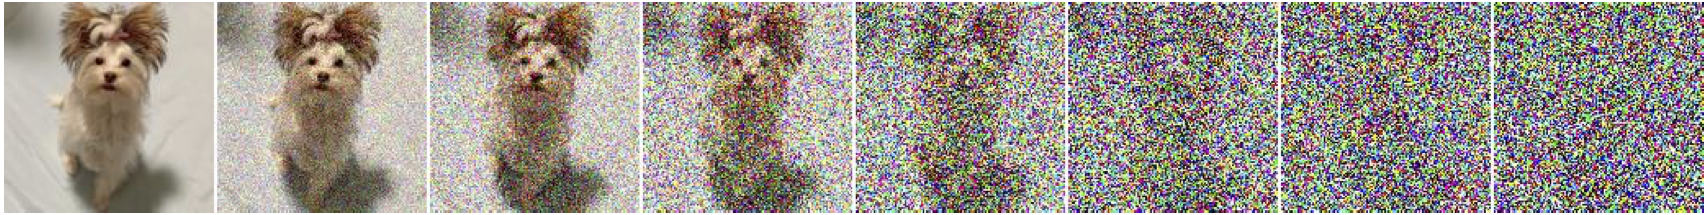
\includegraphics[width=0.86\textwidth]{introduction/figures/diffusion_models/perturbation_sequence.png}
    };

        
    %----------------------------------------------------------------------
    % CONTINUOUS PROCESS (BOTTOM)
    %----------------------------------------------------------------------
    % Node coordinates
    \coordinate (continuousY) at (0,3.5);  % Adjusted vertical level
    \def\XspacingC{17.0}                  % Horizontal spacing for continuous nodes
    
    \node[draw, circle, minimum size=1.4cm] (x0_continuous) 
        at ($(continuousY) + (0,0)$) {$X_0$};
    
    \node[draw, circle, minimum size=1.4cm] (xT_continuous) 
        at ($(xN_discrete) + (0,-5.0)$) {$X_T$};  % Adjusted y-offset
    
    % Forward SDE arrow (straight)
    \draw[->] 
    ([shift={(30:0.7)}]x0_continuous.center) -- 
    node[pos=0.5, above, yshift=0.2em]
    {$\displaystyle dX_t = f(X_t, t)\,dt \;+\; g(t)\,dW_t$}
    ([shift={(150:0.7)}]xT_continuous.center);

    % Reverse SDE arrow (straight)
    \draw[->] 
    ([shift={(210:0.7)}]xT_continuous.center) -- 
    node[pos=0.5, below, yshift=-0.2em]
    {$\displaystyle dX_t = \bigl[f(X_t, t) \;-\; g(t)^2\,\nabla \log p_{X_t}(X_t)\bigr]dt \;+\; g(t)\,d\overline{W}_t$}
    ([shift={(330:0.7)}]x0_continuous.center);
    
    % Label the continuous process
    \node[align=center] (SGM_label) 
        at ($(x0_continuous)!0.5!(xT_continuous) + (0,-2)$)
        {\textbf{Continuous Process (SGM)}};
    
    \end{tikzpicture}
    
    \caption{Illustration of diffusion models in discrete time (DDPM) and continuous time (SGM). DDPM uses a Markov chain to iteratively corrupt data into simple noise and learns a reverse chain to recover it. SGM generalizes this with an SDE that smoothly diffuses data into noise, then reverts it via the reverse SDE. Both methods transform noise into complex data and become equivalent in the limit of infinite steps (\( N \to \infty \)).}
    \label{fig:unified_ddpm_sgm}
\end{figure}




    


    
\textit{Forward Process.} The forward process in diffusion and score-based generative models progressively corrupts the original data into noise, providing the foundation for learning the reverse process that generates data from noise. The design of the forward process ensures that over time, the data distribution transitions smoothly into a simple, analytically tractable distribution $\pi$, such as \( \mathcal{N}(0, \mathbf{I}) \).

\begin{itemize}
    \item \textbf{DDPM (Discrete Time):}
    
    In the Denoising Diffusion Probabilistic Model (DDPM), the forward process is a Markov chain that adds Gaussian noise to the data at discrete time steps \( t = 1, 2, \dots, N \). The transition kernel is given by:
    \[
    q_{X_t \mid X_{t-1}}(\mathbf{x}_t \mid \mathbf{x}_{t-1}) = \mathcal{N}\bigl(\mathbf{x}_t;\, \sqrt{\alpha_t} \, \mathbf{x}_{t-1},\, \beta_t \mathbf{I}\bigr),
    \]
    where:
    \begin{itemize}
        \item \( \alpha_t = 1 - \beta_t \), the scaling factor applied to \( \mathbf{x}_{t-1} \),
        \item \( \beta_t \in (0, 1) \), the predefined variance schedule controlling the amount of noise at step \( t \),
    \end{itemize}
    This formulation allows the process to be expressed in terms of the initial data \( \mathbf{x}_0 \):
    \[
    q_{X_t|X_0}(\mathbf{x}_t \mid \mathbf{x}_0) = \mathcal{N}\left(\mathbf{x}_t;\, \sqrt{\bar{\alpha}_t} \, \mathbf{x}_0,\, (1 - \bar{\alpha}_t) \mathbf{I}\right),
    \]
    where \( \bar{\alpha}_t = \prod_{s=1}^t \alpha_s \) is the cumulative product of \( \alpha_s \). This closed-form expression simplifies training and allows direct sampling from any step \( t \).

    \item \textbf{SGM (Continuous Time):} The forward process in Score-Based Generative Models (SGM) is described by a continuous-time Stochastic Differential Equation (SDE) that progressively perturbs the data distribution with infinitesimal noise:

\[
dX_t = f(X_t, t) \, dt + g(t) \, dW_t,
\]

where:
\begin{itemize}
    \item \( W_t \) is a standard Wiener process (Brownian motion),
    \item \( f(X_t, t) \) is the drift coefficient, defining the deterministic evolution of the data distribution,
    \item \( g(t) \) is the diffusion coefficient, controlling the scale of the stochastic noise.
\end{itemize}

The drift and diffusion coefficients \( f(X_t, t) \) and \( g(t) \) are carefully chosen so that, after a sufficiently large diffusion time \( T \), the data distribution evolves into a distribution that is very close to a simple, analytically tractable distribution, typically the standard normal distribution \( \mathcal{N}(\mathbf{0}, \mathbf{I}) \).

Popular choices for the forward SDE include: 

    
\begin{itemize}
    \item \textbf{Variance Preserving (VP) SDE:}
    \[
    f(X_t, t) = -\frac{1}{2} \beta(t) X_t, \quad g(t) = \sqrt{\beta(t)},
    \]
    where \( \beta(t) \) is a predefined noise schedule that controls the rate of diffusion. This choice preserves the variance of the data distribution throughout the process. The limiting distribution as \( t \to \infty \) is the standard normal distribution. In practice, after sufficient diffusion time \( T \), the perturbed distribution \( p_{X_T} \approx \mathcal{N}(\mathbf{0}, \mathbf{I}) \).
    
    \item \textbf{Variance Exploding (VE) SDE:}
    \[
    f(X_t, t) = \mathbf{0}, \quad g(t) = \sqrt{\frac{d[\sigma^2(t)]}{dt}},
    \]
    where \( \sigma(t) \) is a monotonically increasing function that scales the noise over time. In this formulation, the variance of the data distribution "explodes." After sufficient diffusion time \( T \), the perturbed distribution \( p_{X_T} \approx \mathcal{N}(\mathbf{0}, \sigma(T)^2 \mathbf{I}) \).
\end{itemize}

\end{itemize}

These formulations ensure a smooth progression from the data distribution to the prior, providing a well-defined framework for the reverse process to reconstruct data from noise.


\textit{Reverse Process.} The reverse process reconstructs the original data distribution by inverting the forward process, progressively removing noise to generate data samples:

\begin{itemize}
    \item \textbf{DDPM (Discrete Time):}
    The reverse process in DDPMs is a Markov chain that progressively denoises the data at each step. The conditional distribution for each step is expressed as:
    \[
    p_{X_{t-1} \mid X_t, \theta}(\mathbf{x}_{t-1} \mid \mathbf{x}_t) = \mathcal{N}\bigl(\mathbf{x}_{t-1}; \mu_\theta(\mathbf{x}_t, t), \beta_t^2 \mathbf{I}\bigr),
    \]
    where \( \mu_\theta(\mathbf{x}_t, t) \) is a neural network that predicts the mean of the denoised distribution, given the noisy input \( \mathbf{x}_t \) and the timestep \( t \). Sampling is performed iteratively by drawing from \( p_{X_{t-1} \mid X_t, \theta}(\mathbf{x}_{t-1} \mid \mathbf{x}_t) \), starting with \( \mathbf{x}_T \sim \pi = \mathcal{N}(\mathbf{0}, \mathbf{I}) \).
    \item \textbf{SGM (Continuous Time):}
    In SGMs, the reverse process is governed by the reverse-time SDE, derived from Anderson’s theorem \cite{anderson1982reverse_time_sde}:
    \[
    dX_t = \left[f(X_t, t) - g(t)^2 \nabla_{X_t} \log p_{X_t}(X_t)\right] dt + g(t) \, d\bar{W}_t,
    \]
    where:
    \begin{itemize}
        \item \( \nabla_{X_t} \log p_{X_t}(X_t) \) is the gradient of the log density (score function) of the perturbed distribution at diffusion time \( t \). In practice, the score function is approximated by a neural network \( s_\theta(X_t, t) \), referred to as the score model,
        \item \( \bar{W}_t \) is a reverse-time Wiener process.
    \end{itemize}

    Sampling proceeds by solving this reverse-time SDE, starting from \( X_T \sim \pi \approx p(X_T) \) (e.g., \( \mathcal{N}(\mathbf{0}, \mathbf{I}) \)) and integrating backward from \( t = T \) to \( t = 0 \). This iterative process generates high-quality samples that closely follow the original data distribution.

\end{itemize}

The reverse process lies at the core of diffusion-based generative modeling, enabling the transformation of simple noise into complex data distributions while preserving high fidelity.


\textsc{Training Objective.} Training involves learning to approximate the reverse process by minimizing specific loss functions:

\begin{itemize}
    \item \textbf{DDPM:} In the DDPM framework, the training objective minimizes an expression that upper bounds the negative log-likelihood of the data. This objective is defined as:

    \[
    \mathcal{L}_{\text{DDPM}}(\theta) = \sum_{t=1}^T \mathbb{E}_{X_0 \sim P(X_0),\, \mathbf{E}_t \sim \mathcal{N}(\mathbf{0}, \mathbf{I})} \left[ \bigl\| \mathbf{E}_t - \boldsymbol{\epsilon}_\theta\bigl(\sqrt{\bar{\alpha}_t}\, X_0 + \sqrt{1 - \bar{\alpha}_t}\, \mathbf{E}_t, t\bigr) \bigr\|^2 \right],
    \]

    where:
    \begin{itemize}
        \item \( \mathbf{E}_t \sim \mathcal{N}(\mathbf{0}, \mathbf{I}) \) represents Gaussian noise added at time step \( t \),
        \item \( \boldsymbol{\epsilon}_\theta(\mathbf{x}_t, t) \) is a neural network that estimates the noise component in \(\mathbf{x}_t\),
        \item \( \bar{\alpha}_t = \prod_{s=1}^t \alpha_s \) is the cumulative product of the noise schedule parameters,
        \item \( \alpha_t = 1 - \beta_t \), where \( \beta_t \) is the variance of the noise added at each time step.
    \end{itemize}

    By minimizing \( \mathcal{L}_{\text{DDPM}}(\theta) \), we effectively minimize an upper bound on the negative log-likelihood, enhancing the model's capacity to generate realistic data samples.

    The mean \( \mu_\theta \) of the reverse process used during sampling is derived from the predicted noise \( \mathbf{\epsilon}_\theta \) as follows:
    \[
    \mu_\theta(\mathbf{x}_t, t) = \frac{\sqrt{\bar{\alpha}_{t-1}}\, \beta_t}{1 - \bar{\alpha}_t}\, \hat{\mathbf{x}}_0 + \frac{\sqrt{\alpha_t}\, (1 - \bar{\alpha}_{t-1})}{1 - \bar{\alpha}_t}\, \mathbf{x}_t,
    \]
    where:
    \begin{itemize}
        \item \( \hat{\mathbf{x}}_0 = \frac{\mathbf{x}_t - \sqrt{1 - \bar{\alpha}_t}\, \mathbf{\epsilon}_\theta(\mathbf{x}_t, t)}{\sqrt{\bar{\alpha}_t}} \) is the reconstructed noiseless data point.
    \end{itemize}

    This formulation ensures that the reverse diffusion process effectively removes noise at each step, gradually transforming pure noise into high-quality data samples during generation.


    \item \textbf{SGM:} In the Score-Based Generative Modeling (SGM) framework, the neural network \(s_\theta\) is trained to approximate the \emph{score function} of the perturbed data distribution \(P(X_t)\)—that is, the gradient of its log-density \(\nabla_{\mathbf{x}_t} \log p_{X_t}(\mathbf{x}_t)\). This is achieved by minimizing the weighted \textbf{Denoising Score Matching} objective:
        \[
        \mathcal{L}_{\text{DSM}}(\theta) = \frac{1}{2} \int_0^T \lambda(t) \, \mathbb{E}_{(X_0, X_t) \sim P(X_0, X_t)} \bigl[ \bigl\| s_\theta(X_t, t) - \nabla_{X_t} \log p_{X_t \mid X_0}(X_t \mid X_0) \bigr\|^2 \bigr] \, dt,
        \]

        where:
        \begin{itemize}
            \item \( p_{X_t|X_0}(\mathbf{x}_t \mid \mathbf{x}_0) \) is the perturbation kernel of the forward Stochastic Differential Equation (SDE),
            \item \( \lambda(t) \) is a weighting function,
            \item \( \mathbf{x}_t \) is the diffused data point at time \( t \).
        \end{itemize}

        \citet{song2021maximum} showed that for the particular choice \( \lambda(t) = g(t)^2 \), where \( g(t) \) is the diffusion coefficient of the forward SDE, the \( \mathcal{L}_{\text{DSM}} \) objective serves as an upper bound on the negative log-likelihood.

        In practice, a different weighting function—often referred to as the \emph{simple weighting}—is commonly used:
        \[
        \lambda(t) = \sigma(t)^2,
        \]
        where \( \sigma(t)^2 \) denotes the variance of the forward perturbation kernel \( p_{X_t|X_0}(\mathbf{x}_t \mid \mathbf{x}_0) \). This weighting function has been found to yield superior generative performance, particularly in the image domain where it was initially tested. Consequently, it has become the \emph{de facto} standard for practical implementations.

\end{itemize}

\textsc{Equivalence Between DDPM and SGM.} DDPMs and SGMs are equivalent in the limit as the number of timesteps \( N \to \infty \). Specifically, the forward process in a DDPM converges to the Variance Preserving Stochastic Differential Equation (VP-SDE) used in SGMs:

\[
dX_t = -\tfrac{1}{2} \beta(t) X_t \, dt + \sqrt{\beta(t)} \, dW_t,
\]

\noindent where \( \beta(t) \) is the continuous noise schedule and \( W_t \) is a standard Wiener process. This result is detailed in Song et al.'s paper \textit{Score-Based Generative Modeling through Stochastic Differential Equations} (2020).

\textsc{Probability Flow ODE.} An alternative to the stochastic reverse-time SDE is the \textbf{probability flow ODE}, which provides a deterministic mapping between the data distribution and the prior. The probability flow ODE is defined as:
\[
\frac{d\mathbf{x}_t}{dt} = f(\mathbf{x}_t, t) - \frac{1}{2} g(t)^2 s_\theta(\mathbf{x}_t, t),
\]
where:
\begin{itemize}
    \item \( f(\mathbf{x}_t, t) \) and \( g(t) \) are the drift and diffusion coefficients of the forward SDE,
    \item \( s_\theta(\mathbf{x}_t, t) \) is the approximation of the score function at time \(t\).
\end{itemize}

Under the assumption of a perfectly approximated score function, the probability flow ODE shares the same marginal probability distributions as the reverse-time SDE for all diffusion times. This equivalence arises from considering the Fokker-Planck equations corresponding to both processes, which govern the time evolution of probability densities.

\textit{Computational Efficiency}. In practice, integrating the probability flow ODE has been observed to be computationally more efficient than simulating the reverse-time SDE. Fewer integration steps are typically required to achieve similar sample quality, making it a preferred choice for sampling in diffusion models. This efficiency stems from the deterministic nature of the ODE, which allows for larger step sizes, unlike the stochastic SDE that often requires smaller step sizes to maintain sample fidelity.

\textit{Likelihood Computation with the Probability Flow ODE}. The probability flow ODE enables likelihood computation via the instantaneous change of variables formula. Given the score function \( s_\theta(\mathbf{x}_t, t) \), the log-likelihood of a data point \( \mathbf{x}_0 \) can be expressed as:

\[
\log p_{X_0}(\mathbf{x}_0) = \log p_{X_T}(\mathbf{x}_T) + \int_0^T \nabla_{\mathbf{x}_t} \cdot \mathbf{f}_\theta^{\text{ODE}}(\mathbf{x}_t, t) \, dt,
\]

\noindent where \( \mathbf{f}_\theta^{\text{ODE}}(\mathbf{x}_t, t) \) is the drift term of the probability flow ODE. Direct computation of the divergence term \( \nabla_{\mathbf{x}_t} \cdot \mathbf{f}_\theta^{\text{ODE}}(\mathbf{x}_t, t) \) is often computationally expensive. To address this, the Skilling-Hutchinson trace estimator is used:

\[
\nabla_{\mathbf{x}_t} \cdot \mathbf{f}_\theta^{\text{ODE}}(\mathbf{x}_t, t) \approx \mathbb{E}_{\mathbf{\epsilon} \sim \mathcal{N}(\mathbf{0}, \mathbf{I})} \big[ \mathbf{\epsilon}^\top \nabla_{\mathbf{x}_t} \mathbf{f}_\theta^{\text{ODE}}(\mathbf{x}_t, t) \mathbf{\epsilon} \big],
\]

\noindent where \( \nabla_{\mathbf{x}_t} \mathbf{f}_\theta^{\text{ODE}}(\mathbf{x}_t, t) \) is the Jacobian of \( \mathbf{f}_\theta^{\text{ODE}} \). The term inside the expectation can be efficiently computed using Jacobian-vector product calculations, making this approach both practical and scalable for accurate likelihood computation.


\textsc{Conditional Generation.} Diffusion models can be naturally extended to conditional generation tasks, where the objective is to model the conditional distribution \( p(X_0 \mid C) \), with \( C \) representing the conditioning variable (e.g., class labels, textual descriptions, or other modalities). This extension enables generating data conditioned on specific information, with applications such as super-resolution, inpainting, and text-guided generation.

A widely used approach for conditional generation in diffusion models is the weighted \textbf{Conditional Denoising Score-Matching} (CDSM) objective. The core idea is to train a neural network \( s_\theta(\mathbf{x}_t, \mathbf{c}, t) \) that takes as input the noisy data \( \mathbf{x}_t \), the condition \( \mathbf{c} \), and the time \( t \), and outputs an estimate of the conditional score \( \nabla_{\mathbf{x}_t} \log p_{X_t \mid C}(\mathbf{x}_t \mid \mathbf{c}) \). The training objective is defined as:

\begin{align}
    \mathcal{L}_{\text{CDSM}}(\theta) = 
    \frac{1}{2} \int_0^T \mathbb{E}_{(X_0, X_t, C) \sim p(X_0, X_t, C)} 
    \left[ \lambda(t) \left\| s_\theta(X_t, C, t) - \nabla_{X_t} \log p_{X_t \mid X_0}(X_t \mid X_0) \right\|^2 \right] \, dt.
\end{align}

The only difference between the DSM objective used for unconditional generation and the CDSM objective used for conditional generation lies in the incorporation of the conditioning variable \( C \) into the score model. Note that the regression target—the score function of the perturbation kernel—remains the same. While early empirical results were promising, it was unclear why the minimizer of the CDSM objective approximates the true conditional score function. In chapter \ref{Chapter:non-uniform-diffusion-models}, we provide the first formal proof of consistency for the CDSM estimator, establishing its theoretical validity and confirming its utility in modeling conditional distributions.


\textsc{Strengths.} Diffusion-based generative models have emerged as a powerful class of approaches for learning complex data distributions because they exhibit several notable strengths highlighted across the literature. First, they circumvent many of the pitfalls associated with adversarial training by relying on well-defined, non-adversarial objectives. This design choice reduces issues like mode collapse and training instability that often arise with GANs, leading to more robust and reliable convergence behavior. Second, diffusion models have demonstrated excellent sampling performance in diverse domains—including image, audio, video, and molecule generation—primarily because they do not hinge on stringent architectural constraints (as seen with normalizing flows) or adversarial losses (as with GANs). Their ability to flexibly capture multi-modal and high-dimensional distributions makes them especially appealing when dealing with complex, real-world datasets. Moreover, they derive from well-established stochastic process theory, offering a solid mathematical foundation that guides both theoretical analysis and practical design choices.

\textsc{Weaknesses.} However, one of the most frequently cited weaknesses of diffusion models is their relatively slow sampling speed. The underlying process typically entails running a series of iterative refinement steps—often in the hundreds or thousands—to gradually remove noise and produce high-fidelity samples. This iterative nature translates into significant computational overhead, making diffusion models less suitable for time-critical applications where rapid or real-time generation is paramount. Furthermore, while various techniques have been proposed to reduce sampling time (such as employing fewer refinement steps or adopting improved solvers), these methods usually introduce trade-offs between sample quality and speed.

\textsc{Advancements in Sampling Speed.} Significant progress has been made in accelerating the sampling speed of diffusion models, effectively addressing their primary limitation of slow generation due to iterative steps. A critical observation in this area is that the probability flow ODE, which shares the same marginal distribution as the reverse SDE, is generally preferred for faster sampling. The ODE formulation tends to produce better samples than the corresponding SDE in the low discretization regime \cite{song2020score}. Consequently, many methods that accelerate diffusion models focus on learning to efficiently integrate the probability flow ODE, often as a post-training optimization.

Techniques such as \textbf{Denoising Diffusion Implicit Models (DDIM)} \cite{song2020denoising} reformulate the reverse diffusion process by utilizing non-Markovian dynamics, significantly reducing the number of required sampling steps without compromising sample quality. \textbf{Latent Diffusion Models (LDMs)} \cite{rombach2022high} enhance efficiency by performing diffusion in a compressed latent space, drastically decreasing computational demands while preserving high-resolution outputs. \textbf{Progressive Distillation} \cite{salimans2022progressive} further compresses the multi-step diffusion process into models capable of generating high-fidelity samples in significantly fewer steps—sometimes even a single step. Recently, \textbf{Consistency Models} \cite{song2023consistency} have been introduced, directly mapping noise to data in one step while retaining the advantages of iterative methods.

Collectively, these advancements have significantly reduced sampling times and made diffusion models practical for real-time and interactive applications across various domains.

\section{Self-Supervised Learning}\label{intro:ssl}

\subsection{Motivation}


In today's data-rich environment—spanning social media, sensor outputs, and extensive collections of images, videos and text—the primary challenge is not the lack of data but our ability to utilize it effectively. Despite the vast amounts of information available, much remains unlabeled and underexploited due to the high costs and impracticalities associated with manual labeling. This situation poses a crucial question: \textit{how can we unlock the potential of unlabeled data to develop intelligent systems that learn, adapt, and generalize in a manner akin to human learning?}

Self-supervised learning (SSL) emerges as a compelling approach to this challenge. Referred to by Yann LeCun as the "dark matter of intelligence" \citep{lecun2021self}, SSL enables machines to learn from the abundant unlabeled data by exploiting the inherent structures within it. LeCun remarks:

\begin{quote}
    "Common sense helps people learn new skills without requiring massive amounts of teaching for every single task. Self-supervised learning is one of the most promising ways to build such background knowledge and approximate a form of common sense in AI systems."
\end{quote}

Analogous to how a child learns about the world through observation and pattern recognition rather than explicit instruction, SSL allows models to derive meaningful representations from data without manual labels. The transformative impact of SSL is evident across multiple domains:

\textit{Natural Language Processing (NLP):} SSL has transformed NLP by enabling models to understand and generate human language with improved contextual awareness. Early models like Word2Vec \citep{mikolov2013efficient} and GloVe \citep{pennington2014glove} learned semantic relationships between words through context prediction. Advanced models such as BERT \citep{devlin2019bert} and GPT \citep{radford2019language} employed masked language modeling to pretrain on extensive text corpora, enhancing capabilities in tasks like text completion and machine translation.

\textit{Computer Vision (CV):} In CV, SSL techniques like Contrastive Predictive Coding (CPC) \citep{oord2018representation}, SimCLR \citep{chen2020simple}, and MoCo \citep{he2020momentum} have enabled models to learn visual representations without reliance on labeled datasets. For example, Facebook's SEER model \citep{goyal2021self}, trained on a billion unlabeled images, achieved state-of-the-art performance on ImageNet, illustrating the efficacy of learning from unlabeled visual data.

\textit{Speech Recognition:} SSL models such as wav2vec \citep{schneider2019wav2vec} and wav2vec 2.0 \citep{baevski2020wav2vec} have significantly advanced speech recognition by learning representations from raw audio data. By predicting future audio samples from past ones, these models capture essential phonetic and linguistic features, improving transcription accuracy and the handling of diverse accents and intonations.

\textit{Multimodal Learning:} SSL has significantly advanced the integration of multiple data modalities, enabling AI systems to learn joint representations that bridge the gap between domains like vision, language, and audio. Pioneering models such as CLIP \citep{radford2021learning} have shown remarkable success in aligning images and text within a shared latent space, enabling a wide range of applications. These include image captioning, where the model generates descriptive text for images; text-based image retrieval, allowing users to find images using natural language queries; and zero-shot classification, where the model classifies images into categories it has not seen during training, guided only by textual descriptions.

These advancements are not merely incremental; they signify a fundamental shift in machine learning methodologies. By leveraging unlabeled data, SSL enables models to develop a form of common sense, understanding context and patterns previously inaccessible through supervised learning alone.

The potential applications of SSL are extensive. It opens pathways to developing AI systems capable of understanding and generating human-like language and vision, and learning new tasks with minimal supervision. Self-supervised learning represents a significant step toward creating AI that learns and adapts more like humans, enhancing intelligence and adaptability in artificial systems.


\subsection{Mathematical Formulation of SSL}

Let \(\mathcal{D} = \{\mathbf{x}_i\}_{i=1}^N \subset \mathbb{R}^d\) be a dataset of unlabeled samples, assumed to be drawn i.i.d.\ from an unknown distribution \(P(X)\) over \(\mathbb{R}^d\). The goal of self-supervised learning is to learn an \emph{encoder} function
\[
f_{\theta} : \mathbb{R}^d \to \mathbb{R}^k,
\]
where \(k \le d\), that maps each input \(\mathbf{x} \in \mathbb{R}^d\) into a latent representation \(\mathbf{h} = f_{\theta}(\mathbf{x}) \in \mathbb{R}^k\). These lower-dimensional embeddings act as a concise, informative summary of the original data, improving generalization and serving as a foundation for downstream tasks (e.g., classification, clustering, retrieval).

The encoder \(f_{\theta}\) is parameterized by \(\theta\) and is trained via a \emph{self-supervised loss} function
\[
\theta^* \;=\; \arg\min_{\theta} \mathbb{E}_{X \sim P(X)}\!\bigl[\mathcal{L}(X; \theta)\bigr].
\]
The exact form of \(\mathcal{L}\) depends on the specific SSL approach and typically encourages invariance to augmentations or alignment among related samples. In practice, it may include two or more terms (e.g., a contrastive component plus a regularization term) to jointly enforce closeness of similar samples and separation of dissimilar ones in the latent space.

\subsection{Generative vs. Discriminative SSL}

\begin{forest}
    for tree={
        draw,                          % Draw bounding boxes around each node
        rounded corners,
        align=center,
        edge={-latex},                % Draw edges with an arrow tip
        grow=east,                    % Tree grows horizontally to the right
        parent anchor=east,
        child anchor=west,
        anchor=west,
        font=\footnotesize,           % Reduced font size to fit better
        minimum width=3cm,            % Reduced node width slightly
        minimum height=0.8cm,         % Reduced node height slightly
        l sep+=0.8em,                 % Adjust spacing between levels
        s sep+=0.4em                  % Adjust spacing between siblings
    }
    [SSL
      [\textbf{Discriminative}
        [Pretext Task-Based \\
         (\emph{Rotation, Jigsaw, Temporal Ordering})]
        [Clustering-Based \\
         (\emph{DeepCluster, SwAV})]
        [Feature Decorrelation \\
         (\emph{Barlow Twins, VICReg})]
        [Self-Distillation \\
         (\emph{BYOL, SimSiam})]
        [Contrastive Learning \\
         (\emph{SimCLR, InfoNCE, MoCo})]
      ]
      [\textbf{Generative}
        [\textbf{Masked Distribution}
            [Language Modeling \\
             (\emph{BERT, RoBERTa})]
            [Image Modeling \\
             (\emph{BEiT, MAE})]
        ]
        [\textbf{Full Distribution}
            [GAN-Based \\
             (\emph{StyleGAN, VQ-GAN})]
            [Auto-Encoding \\
             (\emph{VAE, VQ-VAE})]
            [Normalizing Flows \\
             (\emph{FlowGMM})]
            [Auto-Regressive \\
             (\emph{GPT, PixelCNN})]
        ]
      ]
    ]
\end{forest}

Self-supervised learning methods can be broadly categorized into two paradigms: \textbf{generative} and \textbf{discriminative} approaches. Generative methods learn representations by modeling data distributions, while discriminative methods do so by solving auxiliary tasks. This subsection offers a concise overview of both paradigms, emphasizing their distinct characteristics and applications.


\subsubsection{Generative Approaches}

These methods aim to extract meaningful latent representations by modeling the underlying data distribution. These approaches can be broadly categorized into two types based on the scope of the distribution being modeled:
\begin{enumerate}
    \item Full data distribution $P(X)$
    \item Masked data distribution $P(X_{\text{masked}}|X_{\text{context}})$
\end{enumerate}

\paragraph{Learning Latent Representations by Modeling the Full Distribution $p(X)$}

\begin{itemize}
    \item \emph{Auto-Regressive (AR) Models}: Autoregressive (AR) models factorize the data distribution into a product of conditional probabilities, generating each data element sequentially conditioned on the previous ones; for more details, refer to section \ref{sec:auto_regressive_models}.
    \begin{itemize}
        \item \emph{GPT and GPT-2} \citep{radford2019language}: Learn language representations by predicting the next token given preceding context, enabling robust text generation and understanding. GPT embeddings serve as inputs for fine-tuned classifiers in NLP tasks.
        \item \emph{PixelRNN and PixelCNN} \citep{oord2016pixel}: Model pixel dependencies in images for self-supervised representation learning, useful for tasks like image completion. PixelCNN representations have been used in image segmentation.
    \end{itemize}

    \item \emph{Normalizing Flows}: These models transform a simple latent distribution into a complex target distribution through a sequence of invertible mappings, enabling exact computation of likelihoods. For a more detailed explanation, refer to section \ref{sec:normalizing_flows}. Examples include:
\begin{itemize}
    \item \emph{FlowGMM} \citep{izmailov2021flowgmm}: Combines normalizing flows with a Gaussian mixture model in the latent space to extract representations useful for tasks such as text classification, tabular data analysis, and semi-supervised image classification.
\end{itemize}

    \item \emph{Auto-Encoding (AE) Models}: Autoencoders reconstruct data from latent representations, learning robust embeddings for various downstream tasks. Examples include:
    \begin{itemize}
        \item \emph{Variational Autoencoders (VAEs)} \citep{kingma2013auto}: Introduce probabilistic latent spaces, learning smooth representations useful for clustering and semi-supervised learning. For additional details, see section \ref{sec:vae}.
        \item \emph{VQ-VAE} \citep{oord2017neural}: Extends VAEs to discrete latent spaces, providing meaningful representations that have been widely applied in downstream tasks:
        \begin{itemize}
            \item In \textit{audio processing}, VQ-VAE representations have been used in \textit{wav2vec} \citep{baevski2020wav2vec} for unsupervised pretraining on speech data, enabling improvements in downstream speech recognition tasks by learning phonetic and linguistic features from raw audio.
            \item In \textit{vision}, the latent codes are inputs to autoregressive models for image generation, inpainting, and enhancement tasks \citep{razavi2019generating}.
            \item In \textit{multimodal learning}, VQ-VAE representations bridge modalities such as text and images, aiding in tasks like image captioning and cross-modal retrieval \citep{ding2021vqvae}.
        \end{itemize}
    \end{itemize}
    \item \emph{GAN-Based Models}: Generative Adversarial Networks (GANs) learn latent representations by simultaneously training a generator and a discriminator in an adversarial framework; for more details, refer to section \ref{sec:gans}. Recent advancements have adapted GANs for representation learning. Examples include:
    \begin{itemize}
        \item \emph{StyleGAN} \citep{karras2019style}: Generates high-quality images with interpretable latent spaces that enable fine-grained editing (e.g., facial expressions and lighting adjustments). StyleGAN embeddings are widely used in image synthesis and manipulation tasks.
        \item \emph{VQ-GAN} \citep{esser2021taming}: Combines vector quantization and adversarial training to learn discrete latent representations. These representations are used for tasks such as text-to-image generation, image compression, and cross-modal retrieval.
    \end{itemize}
\end{itemize}

\paragraph{Learning Latent Representations by Modeling the Masked Distribution $p(X_{\text{masked}}|X_{\text{context}})$}

\begin{itemize}
    \item \textit{Masked Image Modeling:}
    Models learn representations by reconstructing occluded parts of an image, leveraging context to infer the missing information. Examples include:
        \begin{itemize}
            \item \emph{BEiT} \citep{bao2021beit}: Learns representations for downstream tasks like image classification and segmentation by reconstructing masked patches of images.
            \item \emph{Masked Autoencoders (MAE)} \citep{he2022masked}: Focuses on learning efficient representations by masking a large portion of the input image and reconstructing it from the unmasked portion.
        \end{itemize}
        
        Representations from masked image models are particularly useful for visual tasks such as object detection, segmentation, and classification, where capturing spatial relationships is critical.
    

    \item \textit{Masked Language Modeling:}
    In NLP, masked language models predict missing words or tokens in a sequence, learning rich contextual embeddings. Examples include:
        \begin{itemize}
            \item \emph{BERT} \citep{devlin2019bert}: A foundational model in NLP, pretraining on masked tokens enables fine-tuning for tasks such as sentiment analysis and named entity recognition.
            \item \emph{RoBERTa} \citep{liu2019roberta}: Builds on BERT by optimizing training dynamics and is widely used for text classification and question answering.
        \end{itemize}
        Masked language model representations are extensively used for text-based tasks, including translation, summarization, and retrieval.
\end{itemize}

\subsubsection{Discriminative Approaches}

These methods focus on learning robust feature representations by solving pretext tasks or leveraging contrastive objectives without explicitly modeling the data distribution. The main motivation is to learn representations that are useful for downstream tasks by capturing essential features and invariances in the data. Key techniques include:

\begin{itemize}
    \item \textbf{Contrastive Learning}:
    \begin{itemize}
        \item \emph{Motivation and Logic}: Contrastive learning aims to learn robust feature representations by maximizing agreement between similar pairs (positive pairs) and minimizing agreement between dissimilar pairs (negative pairs). The central idea is to structure the latent space such that representations of similar samples are closer, while representations of different samples are farther apart.

        \item \emph{Training Objective}: The training objective for contrastive learning can be described through a generalized framework that unifies various contrastive losses. \citet{tian2022} proposed a \textit{Generalized Contrastive Loss}, which is expressed as:
        \[
        \mathcal{L}_{\phi,\psi}(\theta) = \sum_{i=1}^{N} \phi \left( \sum_{j \neq i} \psi\left(\|\mathbf{z}_i - \mathbf{z}_j\|_2^2 - \|\mathbf{z}_i - \mathbf{z}_i'\|_2^2\right) \right),
        \]
        where:
        \begin{itemize}
            \item \(\mathbf{z}_i\) and \(\mathbf{z}_i'\) are the representations of a sample \(i\) and its positive pair (e.g. augmented view of the same sample).
            \item \(\|\mathbf{z}_i - \mathbf{z}_j\|_2^2\) is the squared distance between the representations of sample \(i\) and a negative sample \(j\), penalizing similarity to negatives.
            \item \(\|\mathbf{z}_i - \mathbf{z}_i'\|_2^2\) is the squared distance between a sample and its positive pair, promoting positive similarity.
            \item \(\phi\) and \(\psi\) are monotonically increasing and differentiable scalar functions that control how positive and negative distances are weighted.
        \end{itemize}

        \item Examples:
        \begin{itemize}
            \item \emph{InfoNCE Loss} \citep{oord2018representation}: Originally introduced in the context of Contrastive Predictive Coding (CPC), InfoNCE is derived as a variational lower bound on the mutual information between representations of paired samples. Its goal is to learn representations that can discriminate between positive pairs (e.g., correlated views or future contexts of the same signal) and negative pairs (unrelated samples). The form below is a specific instance of the generalized contrastive loss, where \(\phi(x) = \tau \log(\epsilon + x)\) and \(\psi(x) = \exp(x / \tau)\). The hyperparameter \(\tau\) (temperature) controls the separation in the embedding space, and \(\epsilon\) is often chosen as a small positive constant to stabilize the log function:
              \[
                \mathcal{L}_{\text{InfoNCE}} 
                = -\tau \sum_{i=1}^{N} \log 
                \frac{\exp\left(-\|\mathbf{z}_i - \mathbf{z}_i'\|_2^2 / \tau\right)}
                {\epsilon \,\exp\left(-\|\mathbf{z}_i - \mathbf{z}_i'\|_2^2 / \tau\right) 
                + \sum_{j \neq i} \exp\left(-\|\mathbf{z}_i - \mathbf{z}_j\|_2^2 / \tau\right)}.
              \]
              In practice, larger batch sizes (i.e., more negative samples) can significantly improve performance. Furthermore, data augmentations play a critical role in creating meaningful positive pairs for robust representation learning.
        
            \item \emph{SimCLR Loss} \citep{chen2020simple}: Often referred to as the “NT-Xent” loss in the SimCLR framework, this loss is a practical instantiation of InfoNCE with the stabilization term \(\epsilon\) removed (i.e., \(\epsilon = 0\)). SimCLR also leverages strong data augmentations (e.g., random crops, color jittering, Gaussian blur) to create diverse positive pairs for each sample, ensuring the network learns invariances relevant to the downstream task. The resulting loss is:
              \[
                \mathcal{L}_{\text{SimCLR}} 
                = -\tau \sum_{i=1}^{N} \log 
                \frac{\exp\left(-\|\mathbf{z}_i - \mathbf{z}_i'\|_2^2 / \tau\right)}
                {\sum_{j \neq i} \exp\left(-\|\mathbf{z}_i - \mathbf{z}_j\|_2^2 / \tau\right)}.
              \]
              In addition to the loss simplification, SimCLR introduced several design choices—such as careful augmentation strategies, a multi-layer projection head, and larger batch sizes—which further boosted the performance of contrastive self-supervised learning.
        
          \end{itemize}

    \end{itemize}
    \item \textbf{Self-Distillation}:
    \begin{itemize}
        \item \emph{Motivation and Logic}: These methods aim to learn representations without the need for negative samples, addressing issues like the need for large batch sizes or memory banks in contrastive learning. The model learns by predicting its own representations under different augmentations, promoting consistency.
        
        \item \emph{Training Objective}: The model minimizes a prediction loss between representations of different augmented views. For instance, in BYOL, the loss is:
                \[
        \mathcal{L}_{\text{BYOL}} = \left\| \mathbf{q}_i - \text{stopgrad}(\mathbf{z}_i^+) \right\|_2^2,
        \]

        where:
        \begin{itemize}
            \item \( \mathbf{q}_i = f_{\theta}(\mathbf{x}_i) \) is the output of the online network.
            \item \( \mathbf{z}_i^+ = f_{\theta'}(\mathbf{x}_i^+) \) is the output of the target network.
            \item \( \text{stopgrad} \) indicates that gradients are not backpropagated through this path.
            \item \( \theta' \) is an exponential moving average of the parameters \( \theta \).
        \end{itemize}
        
        \item \emph{Examples}:
        \begin{itemize}
            \item \emph{BYOL} \citep{grill2020bootstrap}: Uses an online and a target network to predict one view from another, with the target network updated via an exponential moving average.
            \item \emph{SimSiam} \citep{chen2021exploring}: Simplifies BYOL by removing the momentum encoder and employing a stop-gradient operation to prevent representational collapse.
        \end{itemize}
    \end{itemize}

    \item \textbf{Feature Decorrelation Methods}:
    \begin{itemize}
        \item \emph{Motivation and Logic}: Feature decorrelation methods aim to learn rich and diverse representations by reducing redundancy among feature dimensions. Inspired by Canonical Correlation Analysis (CCA), these approaches encourage each component of the embedding to capture unique information, promoting uncorrelated and informative features. By focusing on decorrelating feature dimensions, these methods prevent representational collapse and enhance the quality of learned representations without relying on negative samples or complex training schemes.
        
        \item \emph{Training Objective}: The central idea is to make embeddings from different augmented views of the same data similar (invariance) while ensuring that different feature dimensions are uncorrelated (decorrelation). This is achieved by combining an invariance term with a decorrelation term in the loss function, encouraging both similarity across views and diversity among features.
        
        \item \emph{Examples}:
        \begin{itemize}
            \item \emph{Barlow Twins} \citep{zbontar2021barlow} employs two identical networks to process different augmented views of the same image. It computes a cross-correlation matrix \( \mathbf{C} \) between the embeddings from the two networks. The loss function encourages the diagonal elements of \( \mathbf{C} \) to be close to one (promoting invariance) and the off-diagonal elements to be close to zero (reducing redundancy):
        
            \[
            \mathcal{L}_{\text{BT}} = \sum_{i=1}^d (1 - \mathbf{C}_{ii})^2 + \lambda \sum_{i \neq j} \mathbf{C}_{ij}^2.
            \]
        
            This approach enables the learning of features that are invariant to augmentations while ensuring each dimension captures distinct information.
        
            \item \emph{VICReg} \citep{bardes2021vicreg} introduces a loss function with three components. The invariance term minimizes the mean squared error between embeddings from different views. The variance term ensures the standard deviation of each feature dimension exceeds a threshold to prevent collapse. The covariance term penalizes off-diagonal covariance elements to reduce redundancy. The loss is expressed as:
        
            \[
            \mathcal{L}_{\text{VICReg}} = \underbrace{\frac{1}{B} \sum_{b=1}^B \| \mathbf{z}_b^{(1)} - \mathbf{z}_b^{(2)} \|_2^2}_{\text{Invariance}} + \gamma \underbrace{\sum_{j=1}^d \max(0, s - \sigma(\mathbf{z})_j)}_{\text{Variance}} + \mu \underbrace{\sum_{i \neq j} \text{Cov}(\mathbf{z})_{ij}^2}_{\text{Covariance}},
            \]
        
            where \( \gamma \) and \( \mu \) balance the terms, \( s \) is the variance threshold, and \( \text{Cov}(\mathbf{z})_{ij} \) is the off-diagonal element of the covariance matrix of \( \mathbf{z} \).
        \end{itemize}        
    \end{itemize}

    \item \textbf{Clustering-Based Methods}:
    \begin{itemize}
        \item \emph{Motivation and Logic}: These approaches leverage unsupervised clustering to group similar data points, learning representations that capture group-level semantic structures. The model alternates between clustering the data in the representation space and updating the encoder to produce features that align with these clusters.
        \item \emph{Training Objective}: The encoder is trained to predict pseudo-labels derived from cluster assignments. The loss function typically involves cross-entropy between the predicted labels and the pseudo-labels:

        \[
        \mathcal{L}_{\text{cluster}} = \sum_{i=1}^N \ell_{\text{CE}}(f_{\theta}(\mathbf{x}_i), y_i),
        \]

        where \( y_i \) is the cluster assignment for \( \mathbf{x}_i \) obtained via a clustering algorithm (e.g., k-means), and \( \ell_{\text{CE}} \) denotes the cross-entropy loss.

        \item \emph{Examples}:
        \begin{itemize}
            \item \emph{DeepCluster} \citep{caron2018deep}: Performs k-means clustering on the learned features and uses the cluster assignments as pseudo-labels for training.
            \item \emph{SwAV} \citep{caron2020unsupervised}: SwAV uses siamese networks to generate embeddings for two augmented views of an image and aligns them with trainable prototypes. It computes cluster assignments online using the Sinkhorn-Knopp algorithm and minimizes cross-entropy between these assignments and predicted probabilities, enabling efficient training without pairwise comparisons.
        \end{itemize}
    \end{itemize}
    \item \textbf{Pretext Task-Based Methods}
    \begin{itemize}
         \item \emph{Motivation and Logic}: Pretext task-based methods aim to learn useful representations by training models on auxiliary tasks where the labels can be derived automatically from the data itself. These tasks, often unrelated to the downstream tasks, encourage the model to capture meaningful patterns and structures in the data that generalize well across applications. By solving these simple yet informative tasks, the model learns features that are transferable to various downstream tasks without requiring manual annotations.

    \item \emph{Examples}:
    \begin{itemize}
        \item \emph{Rotation Prediction} \citep{gidaris2018unsupervised}: The model learns representations by predicting the rotation angle applied to an image. Given an image rotated by one of four angles (\(0^\circ\), \(90^\circ\), \(180^\circ\), or \(270^\circ\)), the model classifies the rotation angle. This task encourages the model to understand spatial relationships and object structures within the image.

        \item \emph{Jigsaw Puzzle Solving} \citep{noroozi2016unsupervised}: The model is tasked with solving jigsaw puzzles by predicting the correct arrangement of shuffled image patches. This pretext task forces the model to learn contextual and semantic relationships between different parts of an image.
        
        \item \emph{Temporal Ordering} \citep{misra2016shuffle}: For video data, the model learns representations by predicting the correct temporal order of video frames. This task helps the model capture temporal dependencies and motion dynamics in videos.
    \end{itemize}
    \end{itemize}

\end{itemize}


\subsubsection{Choosing Between Generative and Discriminative SSL}

The choice between generative and discriminative self-supervised learning methods depends on the specific objectives and requirements of the task. Each approach has its strengths and is more suitable under certain circumstances.

\paragraph{Generative SSL is more useful when:}

Generative SSL methods excel in scenarios that demand a fine-grained understanding of the data distribution. These methods capture detailed and nuanced information within the extracted representations, making them ideal for tasks that require precise and intricate information about the data. For instance, in image editing and manipulation, generative models such as StyleGAN \citep{karras2019style, karras2020analyzing} enable sophisticated modifications by navigating the latent space. By solving optimization problems to move in specific directions within this space, attributes like facial expressions, styles, or lighting conditions can be altered, providing a level of fine-grained control that discriminative models typically cannot offer. Additionally, generative SSL is advantageous in applications like anomaly detection, where understanding the complete data distribution allows for the identification of outliers, and in cross-modal tasks such as text-to-image generation, where translating between different data modalities requires comprehensive distribution modeling.

\paragraph{Discriminative SSL is more useful when:}

Discriminative SSL methods are preferable when the primary goal is to learn efficient, task-relevant representations tailored for specific downstream applications. These methods optimize embeddings to effectively distinguish between different classes or instances, making them highly suitable for tasks such as classification and retrieval. For example, in image classification, discriminative models like SimCLR \citep{chen2020simple} and MoCo \citep{he2020momentum} produce embeddings that enhance performance by focusing on feature discrimination. Furthermore, discriminative SSL is advantageous in environments with limited computational resources, as these methods often require fewer resources and are more scalable. They are also ideal for real-time or latency-sensitive applications, where fast inference and low latency are critical, such as online recommendation systems or real-time monitoring.

\subsubsection{Blurring the Lines: Hybrid Approaches}

The distinction between generative and discriminative SSL methods is increasingly becoming blurred, with hybrid approaches emerging that combine the strengths of both paradigms. These hybrid models leverage the fine-grained distribution modeling of generative methods alongside the efficient, task-specific representation learning of discriminative methods. Notable examples include BEiT \citep{bao2021beit} and iBOT \citep{zhou2022ibot}, which integrate masked image modeling (a generative task) with self-distillation objectives (a discriminative task). By doing so, these models capture rich data representations while maintaining computational efficiency, effectively addressing a broader range of tasks.

  


  


\subsection{Utilizing Learned Representations in Downstream Tasks}

Once the representation function \( f_{\theta} \) is learned, the representations \( \mathbf{h}_i = f_{\theta}(\mathbf{x}_i) \) can be utilized in various downstream tasks. These representations capture essential features and structures in the data, making them valuable inputs for different applications.

\subsubsection{Classification}

In classification problems, the goal is to assign input data to one of several predefined categories. The learned representations \( \mathbf{h}_i \) serve as informative features that can be used to train a classifier. Specifically, we can define a classifier \( g_{\phi} : \mathbb{R}^k \rightarrow \mathbb{R}^C \), where \( C \) is the number of classes, and \( \phi \) represents the parameters of the classifier (e.g., weights of a fully connected layer).

The classifier is trained on a labeled dataset \( \{ (\mathbf{x}_j, y_j) \}_{j=1}^M \), where \( y_j \in \{1, 2, \dots, C\} \) is the class label for sample \( \mathbf{x}_j \). The training involves minimizing a supervised loss function, typically the cross-entropy loss:

\[
\phi^* = \arg \min_{\phi} \frac{1}{M} \sum_{j=1}^M \ell_{\text{CE}}(g_{\phi}(\mathbf{h}_j), y_j),
\]

where \( \mathbf{h}_j = f_{\theta}(\mathbf{x}_j) \) and \( \ell_{\text{CE}} \) denotes the cross-entropy loss function.

The representations \( \mathbf{h}_i \) often capture high-level semantic features and are invariant to variations in the input data that are irrelevant to the classification task, such as changes in lighting, orientation, or background. This invariance leads to better generalization and robustness, improving classification performance even when labeled data is limited.

In practice, the representations can be utilized in two ways:

\begin{itemize}
    \item \textbf{Fixed Feature Extraction}: The encoder \( f_{\theta} \) is kept frozen, and only the classifier \( g_{\phi} \) is trained on the labeled data. This approach is useful when computational resources are limited or when the labeled dataset is small.
    \item \textbf{Fine-Tuning}: Both the encoder \( f_{\theta} \) and the classifier \( g_{\phi} \) are trained (or fine-tuned) jointly on the labeled data. This allows the model to adapt the learned representations to the specific nuances of the downstream task, often leading to better performance.
\end{itemize}

\subsubsection{Other Downstream Tasks}

Similar logic can be applied to other downstream tasks such as object detection, semantic segmentation, instance segmentation, image captioning, and more. In these tasks, the extracted representations \( \mathbf{h}_i \) serve as inputs to task-specific prediction heads. For example, in object detection, the representations can be used to extract feature maps that help in localizing and classifying objects within images. In semantic segmentation, the representations provide spatial and contextual information necessary for assigning class labels to each pixel in an image. For image captioning, the representations capture visual features that can be input to sequence models to generate descriptive captions for images.

In all these tasks, the pretrained encoder \( f_{\theta} \) acts as a feature extractor, and the task-specific prediction heads are trained to perform the desired task using the representations as input. Similar to classification, the encoder \( f_{\theta} \) can be kept fixed or fine-tuned along with the prediction heads. This flexibility allows the model to either leverage the general representations learned during self-supervised pretraining or adapt them to the specific nuances of the downstream task. This approach utilizes the strengths of self-supervised learning to enhance performance across various domains and applications.

\subsection{Challenges and Limitations in Current Methodologies}

Despite significant advancements, current self-supervised learning (SSL) methods face several challenges that hinder their ability to fully capture the underlying structure and complexity of data. In this section, we discuss key weaknesses—particularly those we aim to address in this work—including intrinsic dimension estimation, limited model expressiveness in variational autoencoders (VAEs), and the lack of geometric understanding and interpretability in the latent space.

\subsubsection{Intrinsic Dimension Estimation}

While SSL methods strive to extract meaningful representations from data, they often do not make an informed choice about the latent dimensionality of these representations. Standard practice involves selecting a latent dimension based on convention or precedent in the literature—commonly using values like 512—regardless of the dataset's inherent complexity. This arbitrary selection can lead to suboptimal performance.

If the optimal latent dimension is \( k \) and a significantly larger dimension is chosen, the model may incorporate redundant information in downstream tasks. This redundancy might adversely affect generalization. Conversely, selecting a latent dimension smaller than \( k \) risks losing essential information, leading to reduced performance due to insufficient representation capacity.

Developing methods that can estimate or inform the choice of the intrinsic dimensionality of the data manifold is crucial. Such methods enable models to learn representations that are both efficient and effective, capturing the essential structure of the data without unnecessary complexity.

In chapter \ref{Chapter:intrinsic-dimension}, we present a novel method for estimating the latent dimension using diffusion models trained on the data distribution. We theoretically and experimentally demonstrate that diffusion (or score-based) models inherently encode information about the intrinsic dimensionality. Specifically, we prove that the Jacobian of the score function—modeled by a diffusion or score-based model—captures the low-dimensional intrinsic structure of the data. When data concentrates around a lower-dimensional manifold of dimension \( k \) embedded in a higher-dimensional ambient space of dimension \( d \), the singular value decomposition (SVD) of the Jacobian of the score function yields \( k \) vanishing singular values. This finding provides a principled approach to estimating the intrinsic dimension \( k \) of the data manifold.

\subsubsection{Limited Model Expressiveness in Variational Autoencoders}

Variational autoencoders are widely used in unsupervised representation learning due to their ability to model complex data distributions. However, standard VAEs suffer from limited model expressiveness, primarily attributed to two key assumptions: the encoding distribution (often assumed to be a unimodal Gaussian) and the decoding distribution (also assumed to be a unimodal Gaussian).

The assumption of a Gaussian decoding distribution can lead to blurry reconstructions, especially when modeling complex distributions such as natural images. This limitation arises because a unimodal Gaussian cannot capture the multimodal and intricate structures present in such data. As a result, the learned representations may lack the fine-grained details necessary for high-quality reconstructions and downstream tasks that require precise information.

In chapter \ref{Chapter:ScoreVAE}, we introduce a novel adaptation of the VAE framework called \textit{ScoreVAE}, which addresses this issue by combining a diffusion-time-dependent encoder with an unconditional diffusion model. By employing Bayes' rule for score functions, we analytically derive a robust and flexible model for the reconstruction distribution. Our approach bypasses the unrealistic Gaussian assumption, resulting in a more expressive VAE capable of capturing the complex structures inherent in high-dimensional data like images.

\subsubsection{Geometric Understanding and Interpretability of the Latent Space}

Another significant limitation of current methodologies is the lack of geometric understanding and interpretability in the latent space. Existing methods often fail to effectively exploit the geometry of the data manifold, leading to representations that may not reflect the true relationships and structures within the data. This lack of interpretability hinders our ability to understand and manipulate the latent representations meaningfully.


In chapter \ref{Chapter:Pullback-riemannian-geometry}, we introduce a pullback Riemannian metric induced by the score function, capturing the intrinsic dimensionality and geometry of the data manifold. This enables closed-form geodesics, interpretable autoencoding, and a deeper understanding of the manifold's structure. By adapting the normalizing flow framework with isometry regularization and base distribution anisotropy, our method preserves local manifold properties, facilitates dimensionality reduction, and enhances the interpretability of latent space representations.
